\documentclass[11pt,a4paper]{article}

\usepackage[utf8]{inputenc}
\usepackage[T1]{fontenc}
\usepackage[spanish]{babel}
\usepackage[margin=2.5cm]{geometry}
\usepackage{mathptmx}
\usepackage{amsmath}
\usepackage{amssymb}
\usepackage{graphicx}
\usepackage{caption}
\usepackage{float}

\renewcommand{\vec}[1]{\mathbf{#1}}

\begin{document}

% ---------------------------------------------------------------------
% Portada
% ---------------------------------------------------------------------
\begin{titlepage}
\centering
\vspace*{2cm}
{\Large Simulación de Sistemas\par}
\vspace{0.5cm}
{\LARGE\bfseries Trabajo Práctico 2\par}
\vspace{0.3cm}
{\large Autómata off-lattice: bandadas de agentes autopropulsados\par}
\vspace{2cm}
{\large
Grupo: G6\par
Comisión: S2\par
Integrantes: Franco Ferrari, Mateo Pirola y Katia Menshikoff\par
Fecha de entrega: 04/09/2026\par
}
\vfill
\end{titlepage}

\tableofcontents
\newpage

% ---------------------------------------------------------------------
\section{Introducción}
% ---------------------------------------------------------------------

El objetivo del trabajo fue estudiar la formación de orden colectivo en sistemas de partículas autopropulsadas. Este tipo de sistemas aparece como modelo simplificado de bandadas, cardúmenes o colonias bacterianas, donde cada individuo responde solo a información local pero el conjunto puede desarrollar un comportamiento macroscópico organizado.

El problema se abordó mediante un modelo off-lattice: las partículas se mueven en posiciones continuas dentro de una caja cuadrada con condiciones periódicas de contorno. Cada partícula tiene una dirección de movimiento y una rapidez fija; la evolución temporal combina interacción con vecinos cercanos y ruido angular. De esta forma, el parámetro de ruido permite estudiar la competencia entre alineación local y desorden.

Se compararon dos reglas microscópicas de interacción. En el modelo de Vicsek, cada partícula actualiza su dirección a partir del promedio de las orientaciones de sus vecinos. En el modelo de votante, en cambio, copia la orientación de un único vecino elegido al azar. La comparación entre ambos modelos permite analizar cómo cambia el orden global cuando se modifica solamente la regla local de orientación, manteniendo iguales la geometría, los parámetros físicos y el protocolo estadístico.

% ---------------------------------------------------------------------
\section{Modelo e implementación}
% ---------------------------------------------------------------------

El sistema se representó mediante $N$ partículas puntuales en una caja cuadrada periódica de lado $L$. Cada partícula $i$ posee una posición continua $\vec{x}_i(t) = (x_i(t), y_i(t))$ y una orientación $\theta_i(t)$. La rapidez individual se mantiene constante e igual a $v$, por lo que la velocidad queda determinada por

\begin{equation}
\vec{v}_i(t) = v\,\big(\cos\theta_i(t),\ \sin\theta_i(t)\big).
\label{eq:velocidad}
\end{equation}

Los parámetros fijos utilizados fueron $L=10$, $r_c=1$, $\Delta t=1$ y $v=0.03$. Las posiciones iniciales se tomaron uniformemente en la caja y las orientaciones iniciales de manera uniforme en el intervalo $[0,2\pi)$.

La posición se actualiza con la velocidad del instante actual,

\begin{equation}
\vec{x}_i(t+\Delta t) = \vec{x}_i(t) + \vec{v}_i(t)\,\Delta t.
\label{eq:posicion}
\end{equation}

Luego de mover las partículas se aplican condiciones periódicas de contorno. Esto evita introducir paredes o bordes físicos: una partícula que sale por un lado de la caja vuelve por el lado opuesto. La misma periodicidad se usa para calcular distancias entre partículas, de modo que dos partículas próximas a bordes opuestos pueden ser vecinas.

La vecindad se definió mediante un radio de interacción $r_c$. Dos partículas se consideran vecinas si su distancia mínima periódica $d_{ij}(t)$ satisface

\begin{equation}
d_{ij}(t) \le r_c.
\label{eq:vecindad}
\end{equation}

Para acelerar esta búsqueda se implementó el Cell Index Method (CIM), que divide la caja en celdas y restringe las comparaciones a la celda propia y las celdas adyacentes. Con los parámetros del TP, $L=10$ y $r_c=1$, la caja queda dividida en una grilla de $10\times10$ celdas. Esta implementación se validó contra una búsqueda por fuerza bruta, que compara todos los pares de partículas.

En el modelo de Vicsek~[1], la orientación nueva se obtiene promediando vectorialmente las direcciones de los vecinos dentro del radio de interacción, incluida la propia partícula:

\begin{equation}
\theta_i(t+\Delta t) = \operatorname{atan2}\!\left(\ \sum_{j \in \mathcal{N}_i(t)\cup\{i\}} \sin\theta_j(t),\ \ \sum_{j \in \mathcal{N}_i(t)\cup\{i\}} \cos\theta_j(t)\ \right) + \xi_i(t).
\label{eq:vicsek}
\end{equation}

Este promedio se realiza sobre senos y cosenos, y no directamente sobre los ángulos, para evitar errores asociados a la periodicidad angular.

En el modelo de votante~[2] se mantuvo la misma geometría, el mismo movimiento y el mismo ruido, pero se reemplazó la regla de orientación. Si la partícula $i$ tiene vecinos externos, elige uno de ellos al azar y copia su orientación:

\begin{equation}
\theta_i(t+\Delta t) = \theta_{j_i}(t) + \xi_i(t), \qquad j_i \sim \text{Uniforme}\big(\mathcal{N}_i^{*}(t)\big),
\label{eq:votante}
\end{equation}

donde $\mathcal{N}_i^{*}(t) = \{\, j \neq i : d_{ij}(t) \le r_c \,\}$ excluye a la propia partícula. Si no hay otro vecino dentro del radio de interacción, la partícula conserva su orientación anterior y solo se le suma el ruido.

En ambos modelos el ruido angular se tomó uniforme,

\begin{equation}
\xi_i(t) \sim \mathcal{U}\!\left[-\frac{\eta}{2},\ \frac{\eta}{2}\right].
\label{eq:ruido}
\end{equation}

La actualización se realizó de manera sincrónica: todas las partículas calculan sus nuevas orientaciones a partir del mismo estado en tiempo $t$, sin usar valores ya actualizados de otras partículas. Además, el movimiento de las posiciones se hace con $\vec{v}_i(t)$ (Ec.~\ref{eq:posicion}), no con $\vec{v}_i(t+\Delta t)$. Recién al final del paso temporal se reemplaza el estado completo por el nuevo estado.

El motor de simulación se implementó en C++. La salida se guardó en archivos de texto, principalmente \texttt{observables.csv} y, cuando fue necesario, \texttt{trajectory.csv}. Esta separación permite que las mediciones, los gráficos y las animaciones se generen a partir de archivos producidos por el motor, sin depender del tiempo de ejecución de la simulación.

% ---------------------------------------------------------------------
\section{Simulaciones y protocolo}
% ---------------------------------------------------------------------

\subsection{Protocolo del estudio de polarización}

El observable principal fue la polarización, definida como

\begin{equation}
v_a(t) = \frac{1}{N v} \left| \sum_i \vec{v}_i(t) \right|.
\label{eq:va}
\end{equation}

donde $N$ es el número de partículas y $v$ es el módulo constante de la velocidad individual. El observable toma valores entre $0$ y $1$: valores próximos a $1$ indican que las direcciones están alineadas y valores próximos a $0$ corresponden a un estado globalmente desordenado.

Se estudiaron las densidades $\rho = 2$, $4$ y $8$, equivalentes a $N = 200$, $400$ y $800$ partículas en una caja cuadrada periódica de lado $L = 10$. Para cada combinación de modelo, densidad y ruido $\eta$ se realizaron $20$ simulaciones independientes de $3000$ pasos. El valor estacionario de cada realización se obtuvo promediando la serie temporal en el intervalo $t = 1500$ a $3000$; posteriormente se promedió entre realizaciones. La línea vertical presente en las series temporales indica el comienzo de esta ventana, $t_{eq} = 1500$.

Las barras de error de las curvas estacionarias y las bandas sombreadas de las series temporales representan el desvío estándar entre las $20$ realizaciones. Por lo tanto, expresan la dispersión observada entre corridas independientes y no el error estándar de la media.

% ---------------------------------------------------------------------
\section{Resultados}
% ---------------------------------------------------------------------

\subsection{Polarización en el modelo de Vicsek}

La Fig.~\ref{fig:1} muestra configuraciones características para $\rho = 2$ en el instante $t = 2000$. Con $\eta = 1$, las partículas presentan direcciones similares y se observan regiones que se desplazan de manera coherente; por ello, la polarización es alta. En contraste, para $\eta = 5$ las direcciones cubren gran parte del rango angular y la polarización disminuye marcadamente. La comparación visual ilustra que el aumento del ruido compite con la alineación obtenida al promediar las direcciones de los vecinos.

\begin{figure}[H]
\centering
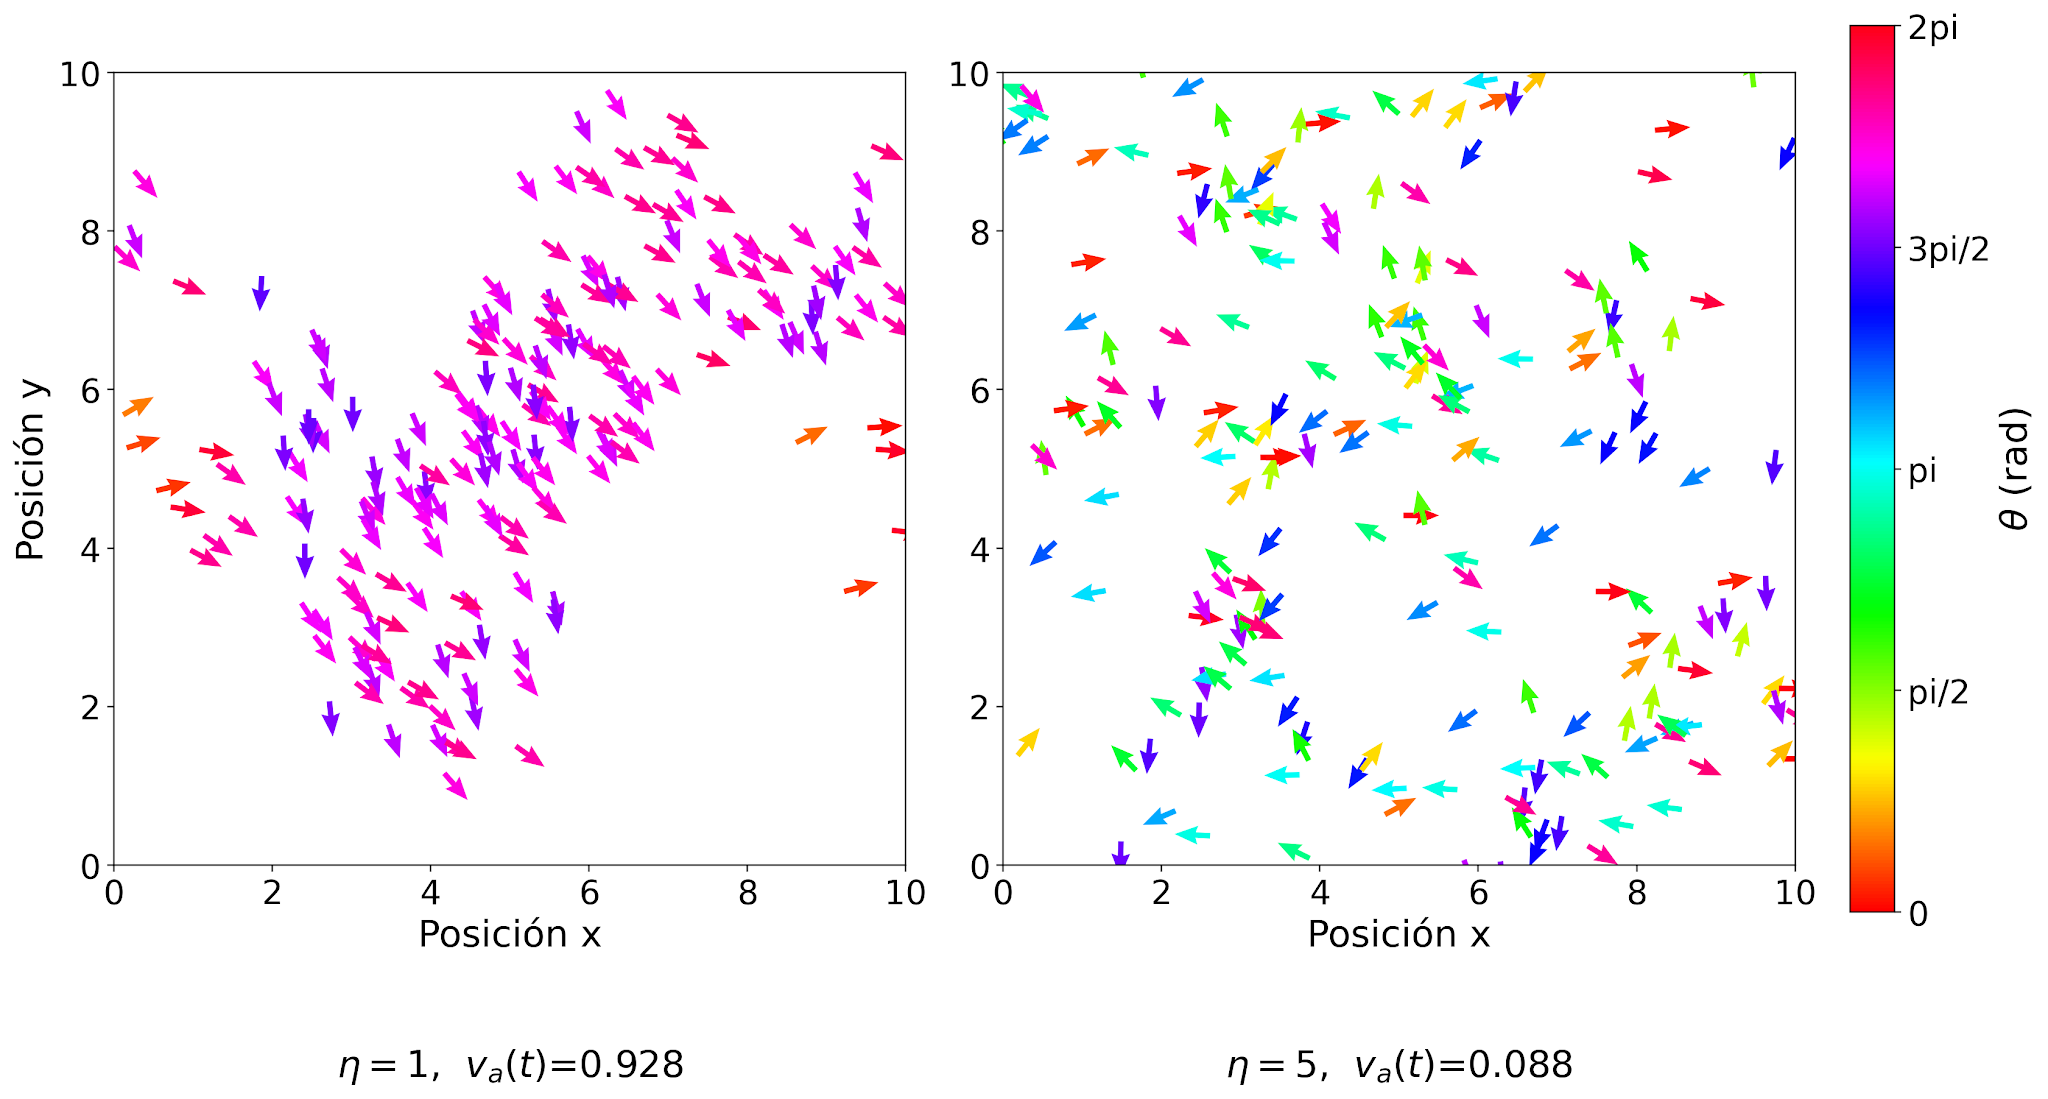
\includegraphics[width=0.85\linewidth]{figs/image1.png}
\caption{Configuraciones del modelo de Vicsek para $\rho = 2$ y $t = 2000$. Panel izquierdo: $\eta = 1$. Panel derecho: $\eta = 5$.}
\label{fig:1}
\end{figure}

El observable $S$, definido como la fracción de partículas de la componente conexa más grande, se presenta en la Sección~\ref{sec:clusters}.

La evolución temporal de $v_a$ para $\rho = 2$ se presenta en la Fig.~\ref{fig:2}. Para $\eta = 1$, el sistema alcanza rápidamente una polarización alta, cercana a $0.92$, y la mantiene a lo largo de la simulación. Para $\eta = 3$, la polarización se estabiliza en un valor intermedio, alrededor de $0.45$, con fluctuaciones entre realizaciones claramente mayores. Con $\eta = 5$, el valor de $v_a$ permanece bajo, cercano a $0.07$, porque el ruido impide sostener una dirección colectiva. El régimen intermedio evidencia la competencia entre alineación y ruido, pero estas simulaciones no permiten estimar un punto crítico ni el orden de una transición.

\begin{figure}[H]
\centering
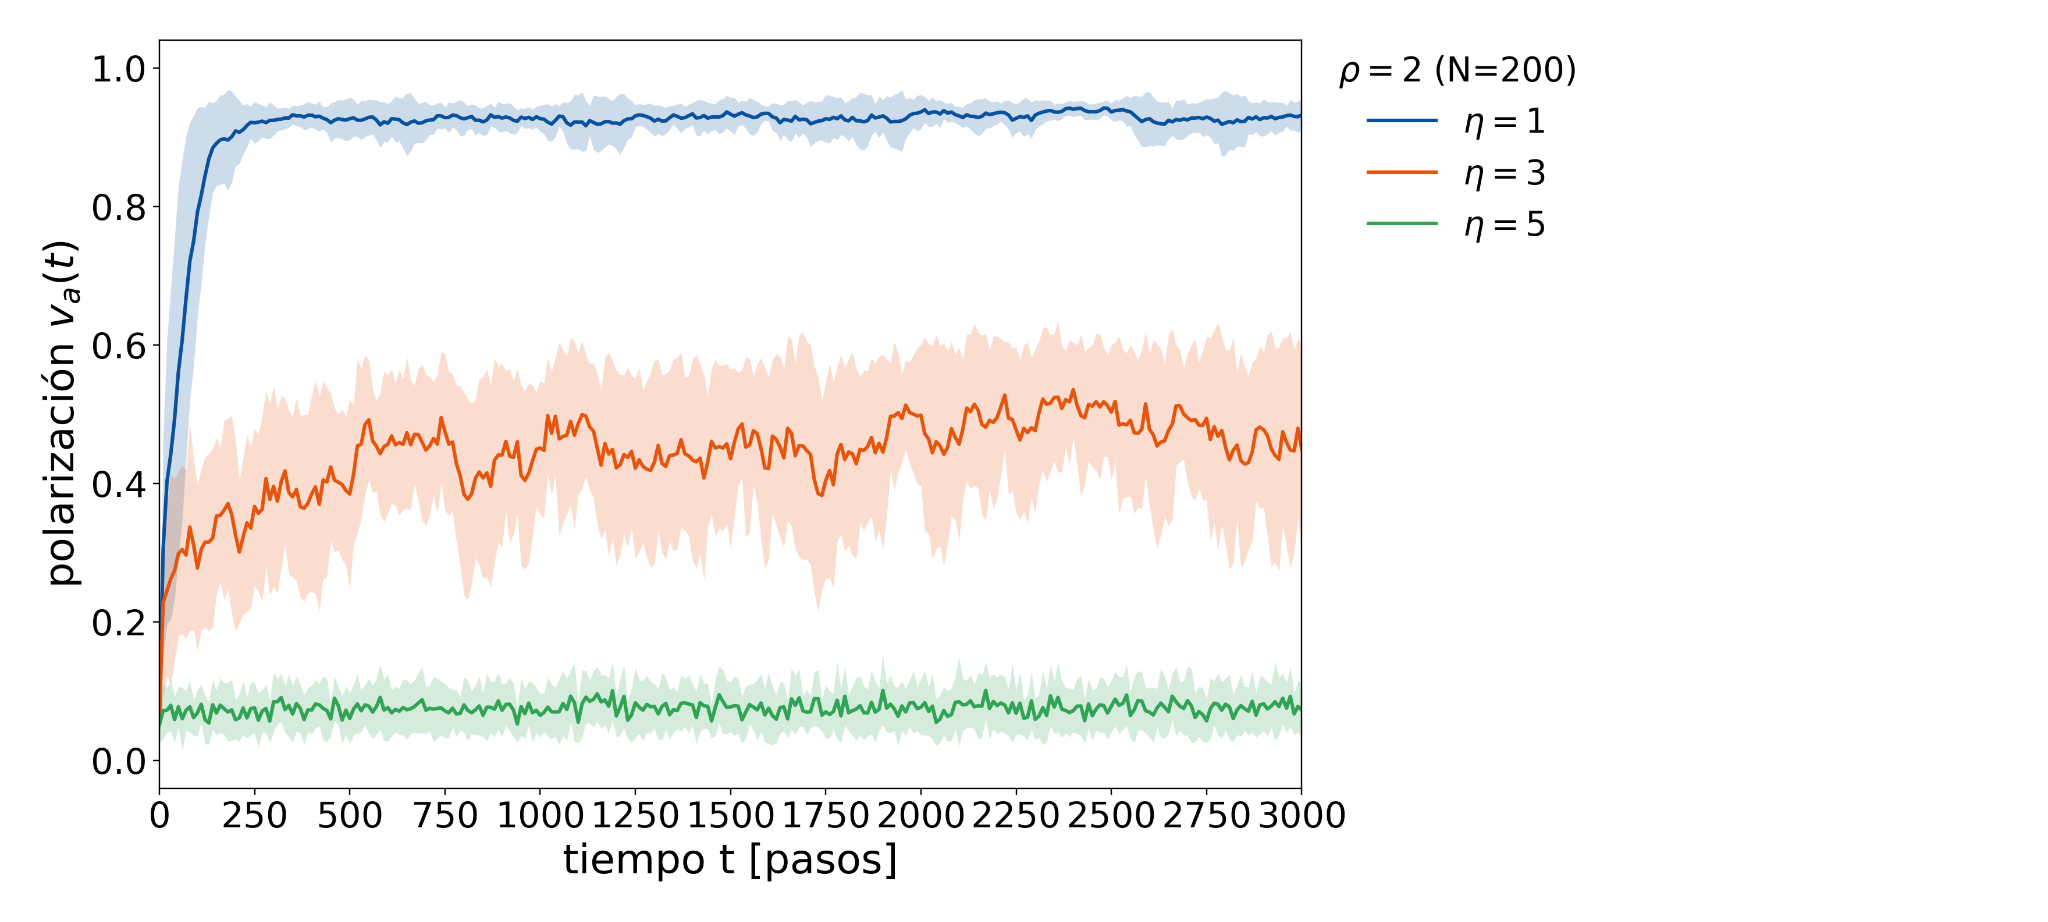
\includegraphics[width=0.85\linewidth]{figs/image2.png}
\caption{Evolución temporal de la polarización en el modelo de Vicsek para $\rho = 2$. Se muestran $\eta = 1$, $3$ y $5$; las bandas representan un desvío estándar entre realizaciones.}
\label{fig:2}
\end{figure}

La Fig.~\ref{fig:3} reúne los promedios estacionarios para las tres densidades. En todos los casos, la polarización disminuye al aumentar $\eta$. Además, en la mayor parte del intervalo de ruido, las densidades más altas conservan una polarización mayor. Este resultado es consistente con la regla de Vicsek: al aumentar la cantidad de vecinos, el promedio vectorial integra más direcciones y atenúa las fluctuaciones individuales. Para ruido alto, todas las curvas convergen a valores bajos y las diferencias entre densidades pierden relevancia.

\begin{figure}[H]
\centering
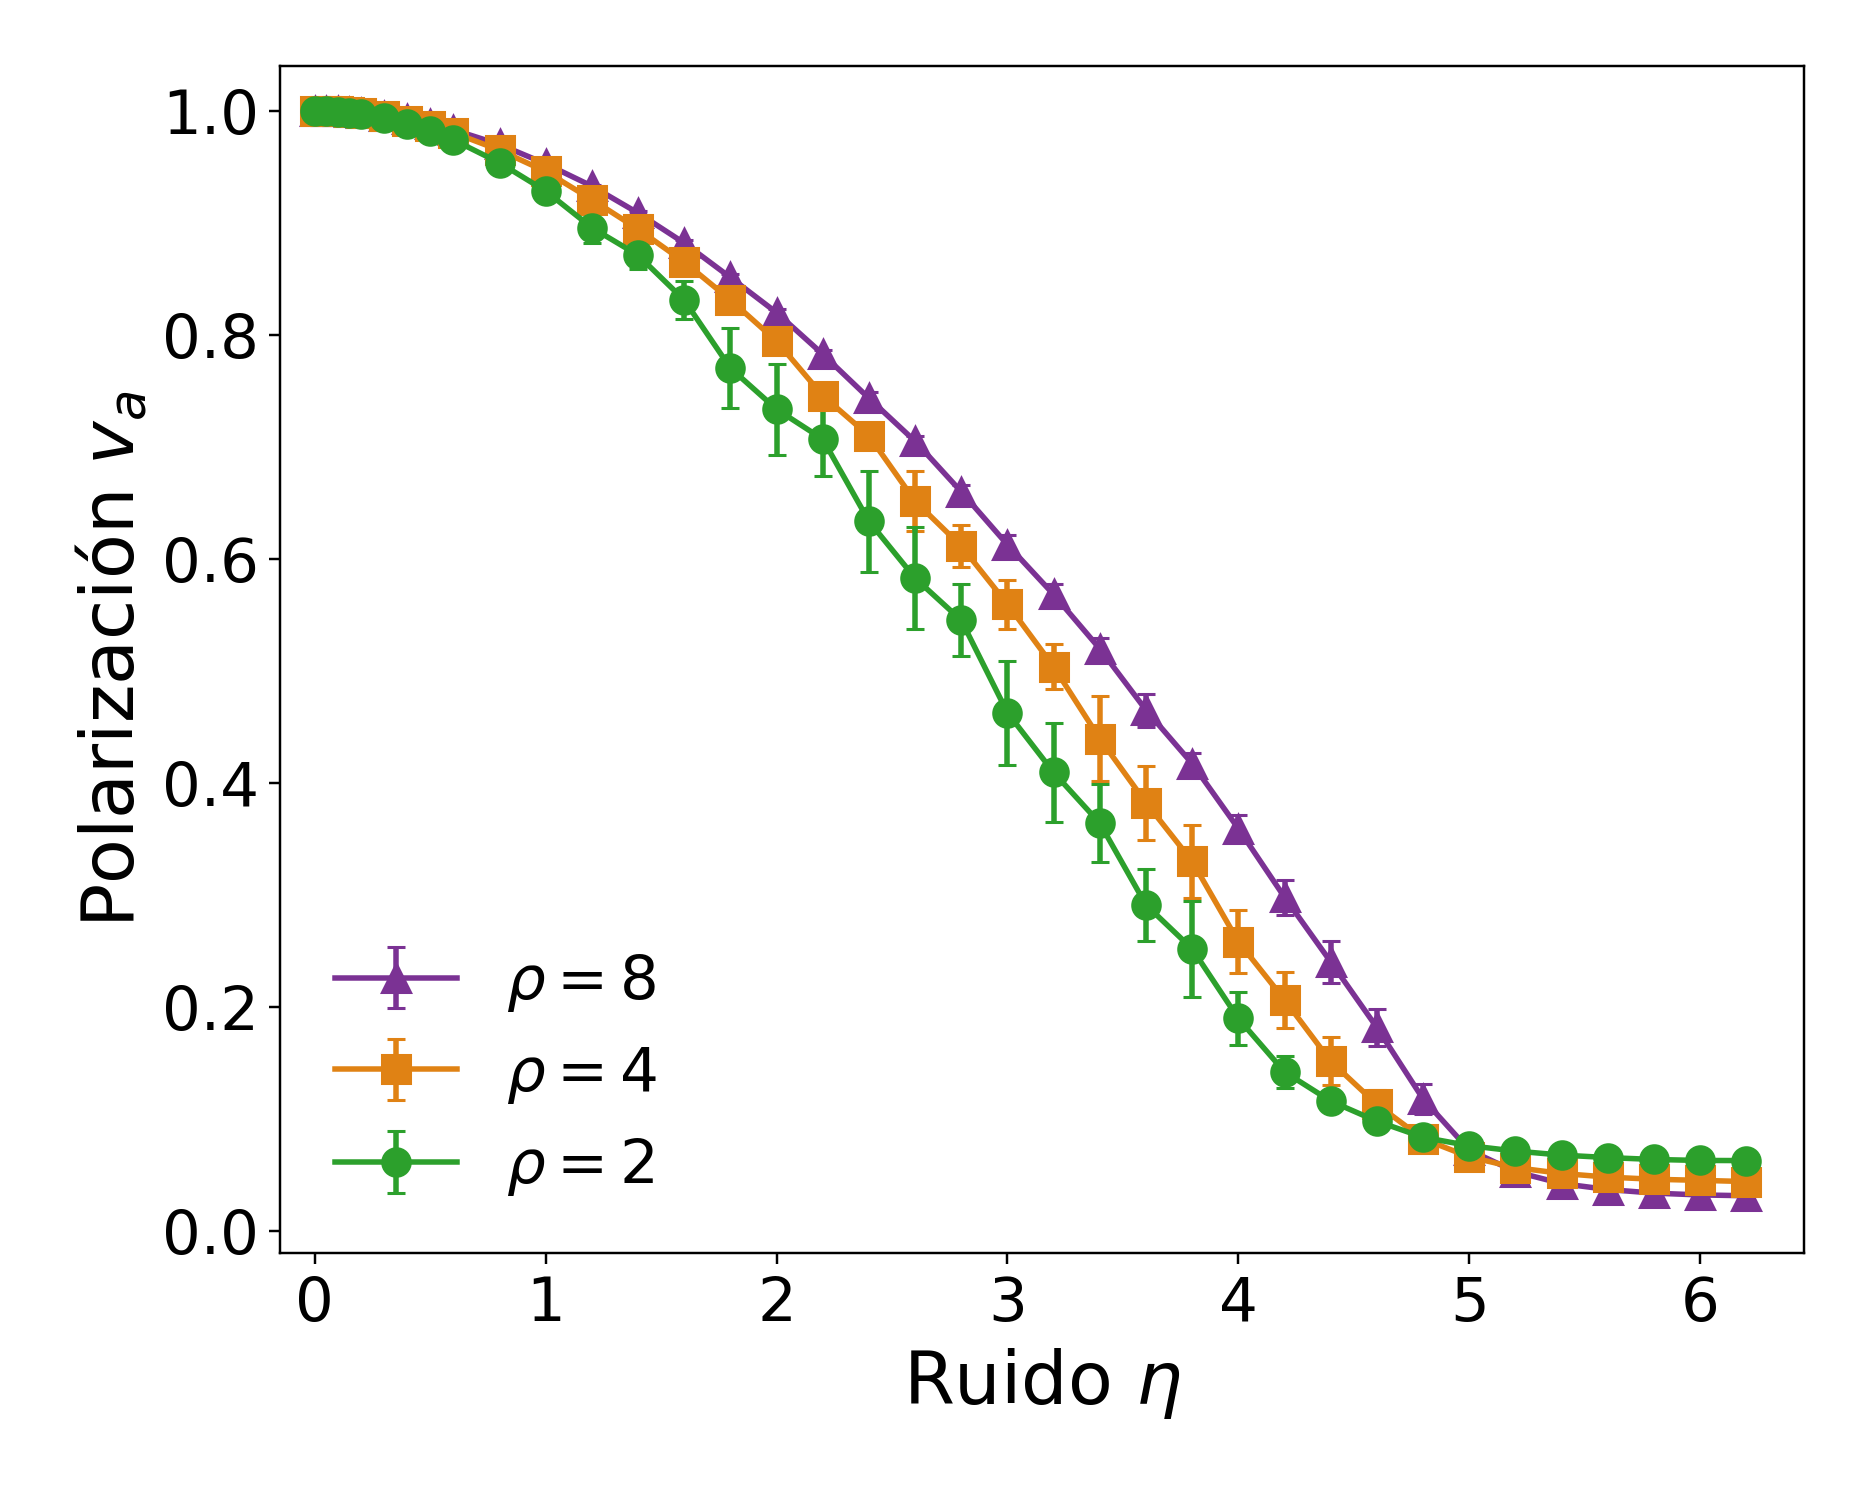
\includegraphics[width=0.85\linewidth]{figs/image3.png}
\caption{Polarización estacionaria en función del ruido para el modelo de Vicsek y $\rho = 2$, $4$ y $8$. Cada punto es el promedio temporal estacionario de una realización, promediado luego sobre $20$ realizaciones; las barras indican desvío estándar entre realizaciones.}
\label{fig:3}
\end{figure}

\subsection{Polarización en el modelo de votante}

En el modelo de votante cada partícula copia la orientación de un único vecino elegido al azar, en lugar de promediar todas las direcciones disponibles. Esta diferencia se refleja en la mayor sensibilidad al ruido. La Fig.~\ref{fig:4} presenta dos configuraciones a $\rho = 2$ y $t = 2000$. Para $\eta = 0.1$ se observa una orientación colectiva marcada, con $v_a(t) = 0.973$; al aumentar el ruido a $\eta = 1$, la distribución angular se vuelve más heterogénea y la polarización global disminuye a $v_a(t) = 0.354$.

\begin{figure}[H]
\centering
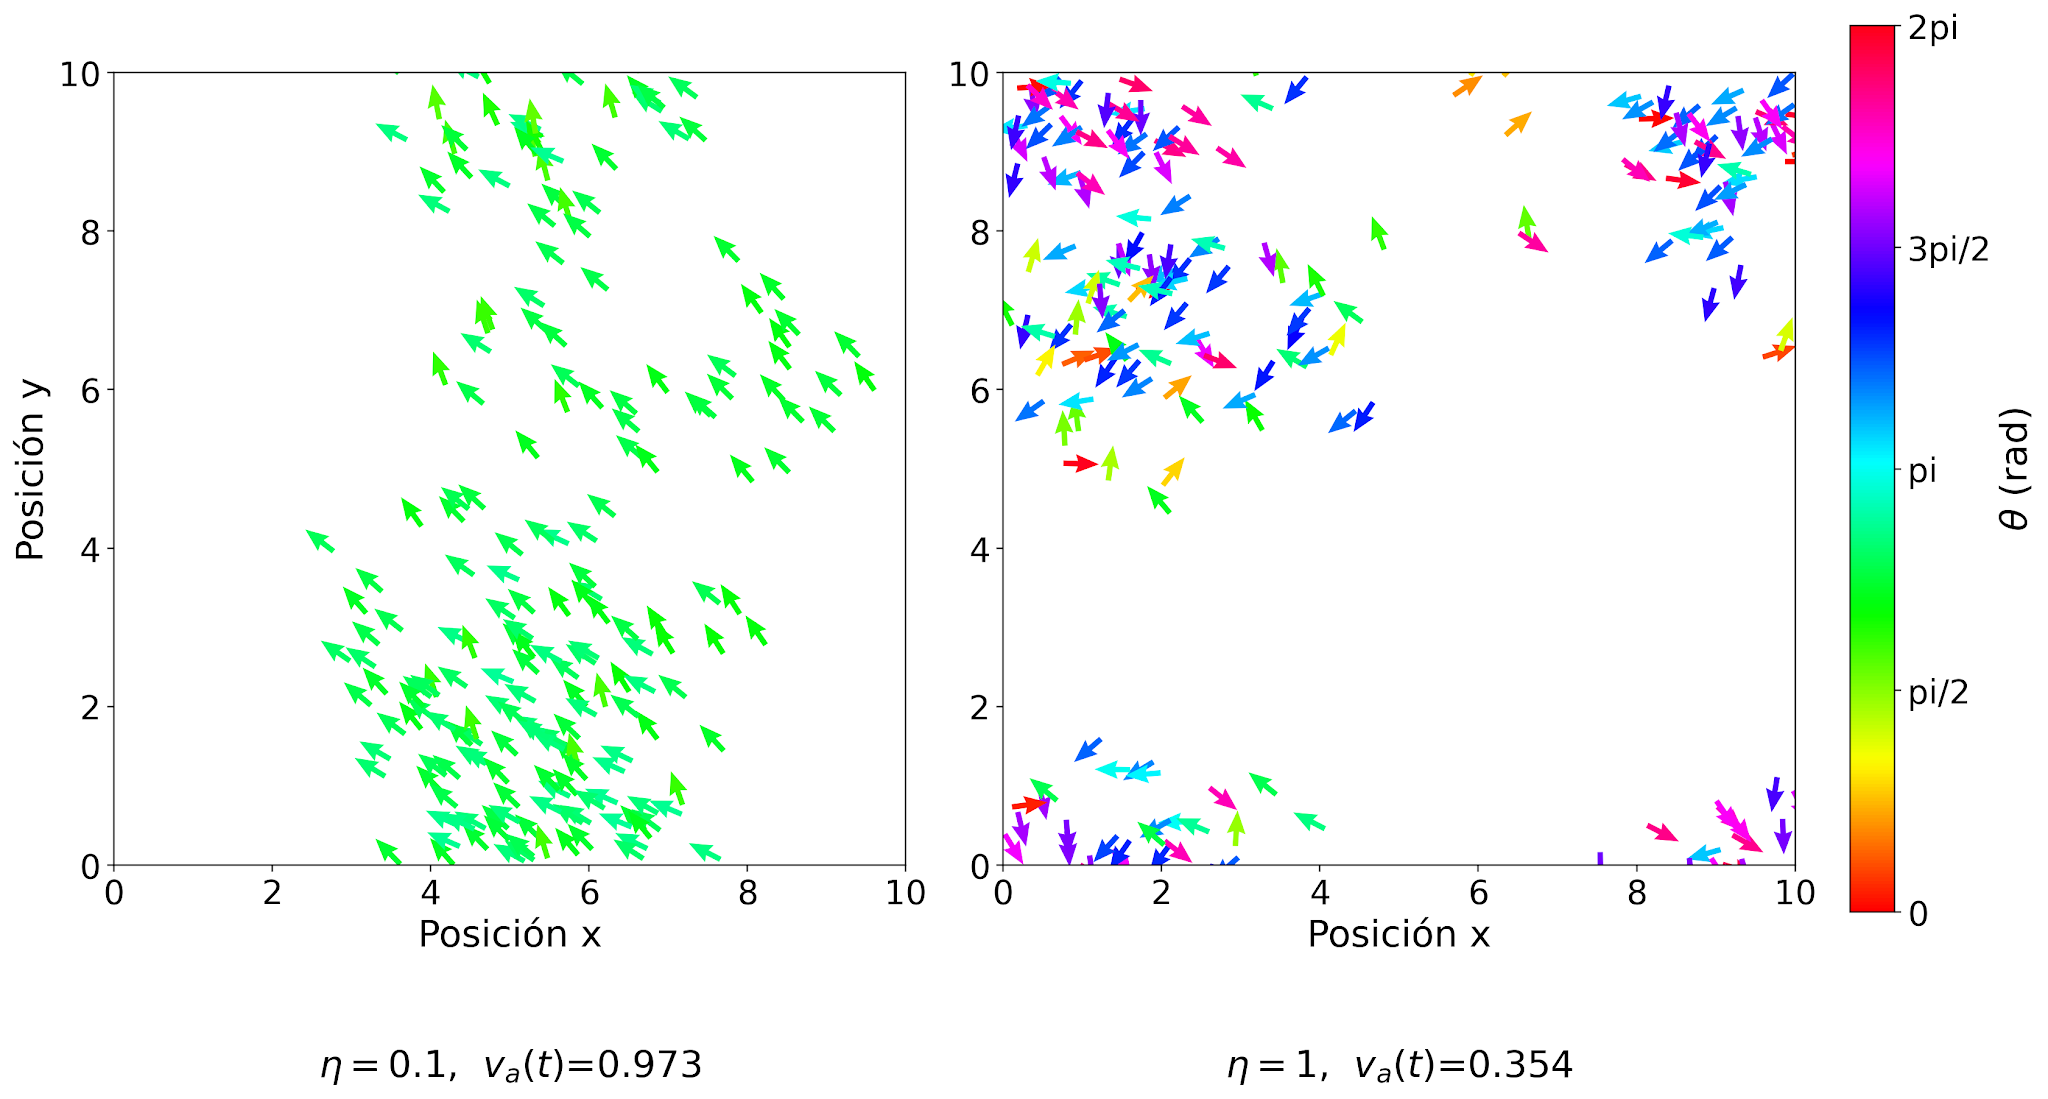
\includegraphics[width=0.85\linewidth]{figs/image4.png}
\caption{Configuraciones del modelo de votante para $\rho = 2$ y $t = 2000$. Panel izquierdo: $\eta = 0.1$ y $v_a(t) = 0.973$. Panel derecho: $\eta = 1$ y $v_a(t) = 0.354$.}
\label{fig:4}
\end{figure}

La Fig.~\ref{fig:5} muestra la evolución temporal para la misma densidad. Con $\eta = 0.05$, el sistema alcanza un estado altamente polarizado, cercano a $v_a = 0.97$, aunque presenta una dispersión inicial apreciable entre realizaciones. Para $\eta = 0.3$, la polarización permanece en un régimen intermedio, alrededor de $0.55$, con fluctuaciones amplias. Con $\eta = 1$, el valor de $v_a$ se mantiene bajo, alrededor de $0.20$. Estas fluctuaciones reflejan que, en la región intermedia, las correlaciones locales se forman y se destruyen continuamente; no constituyen por sí solas una demostración de una transición de fase.

\begin{figure}[H]
\centering
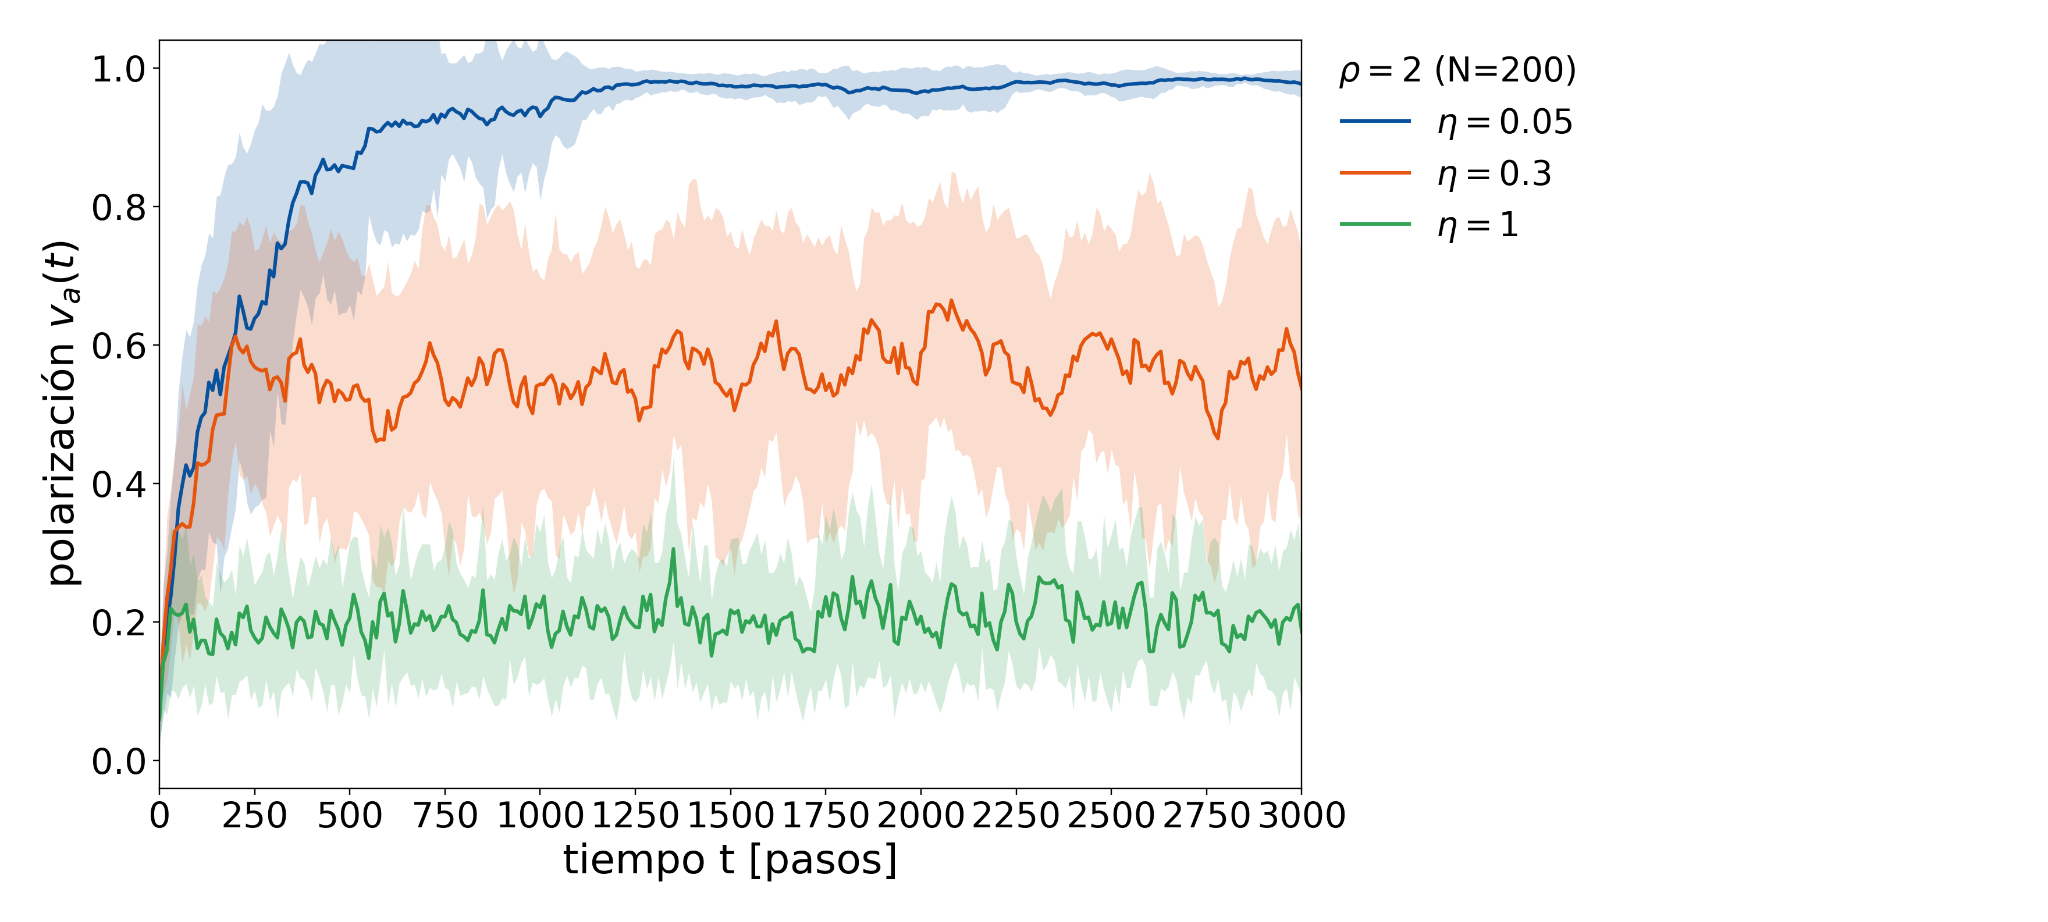
\includegraphics[width=0.85\linewidth]{figs/image5.png}
\caption{Evolución temporal de la polarización en el modelo de votante para $\rho = 2$. Se muestran $\eta = 0.05$, $0.3$ y $1$; las bandas representan un desvío estándar entre realizaciones.}
\label{fig:5}
\end{figure}

La caída de la polarización con $\eta$ es mucho más abrupta en la Fig.~\ref{fig:6}. A diferencia de Vicsek, para el votante la densidad mayor no se asocia a una polarización estacionaria mayor: en las simulaciones, $\rho = 2$ conserva valores de $v_a$ superiores a $\rho = 4$ y $\rho = 8$ en buena parte del régimen de ruido bajo e intermedio. Este ordenamiento es un resultado empírico del modelo bajo el protocolo utilizado. Una explicación posible es que copiar una sola dirección no realiza el filtrado de fluctuaciones que produce el promedio vectorial; no obstante, el estudio no separa de manera independiente los efectos de densidad y tamaño $N$, por lo que no se atribuye una causa única al comportamiento observado.

\begin{figure}[H]
\centering
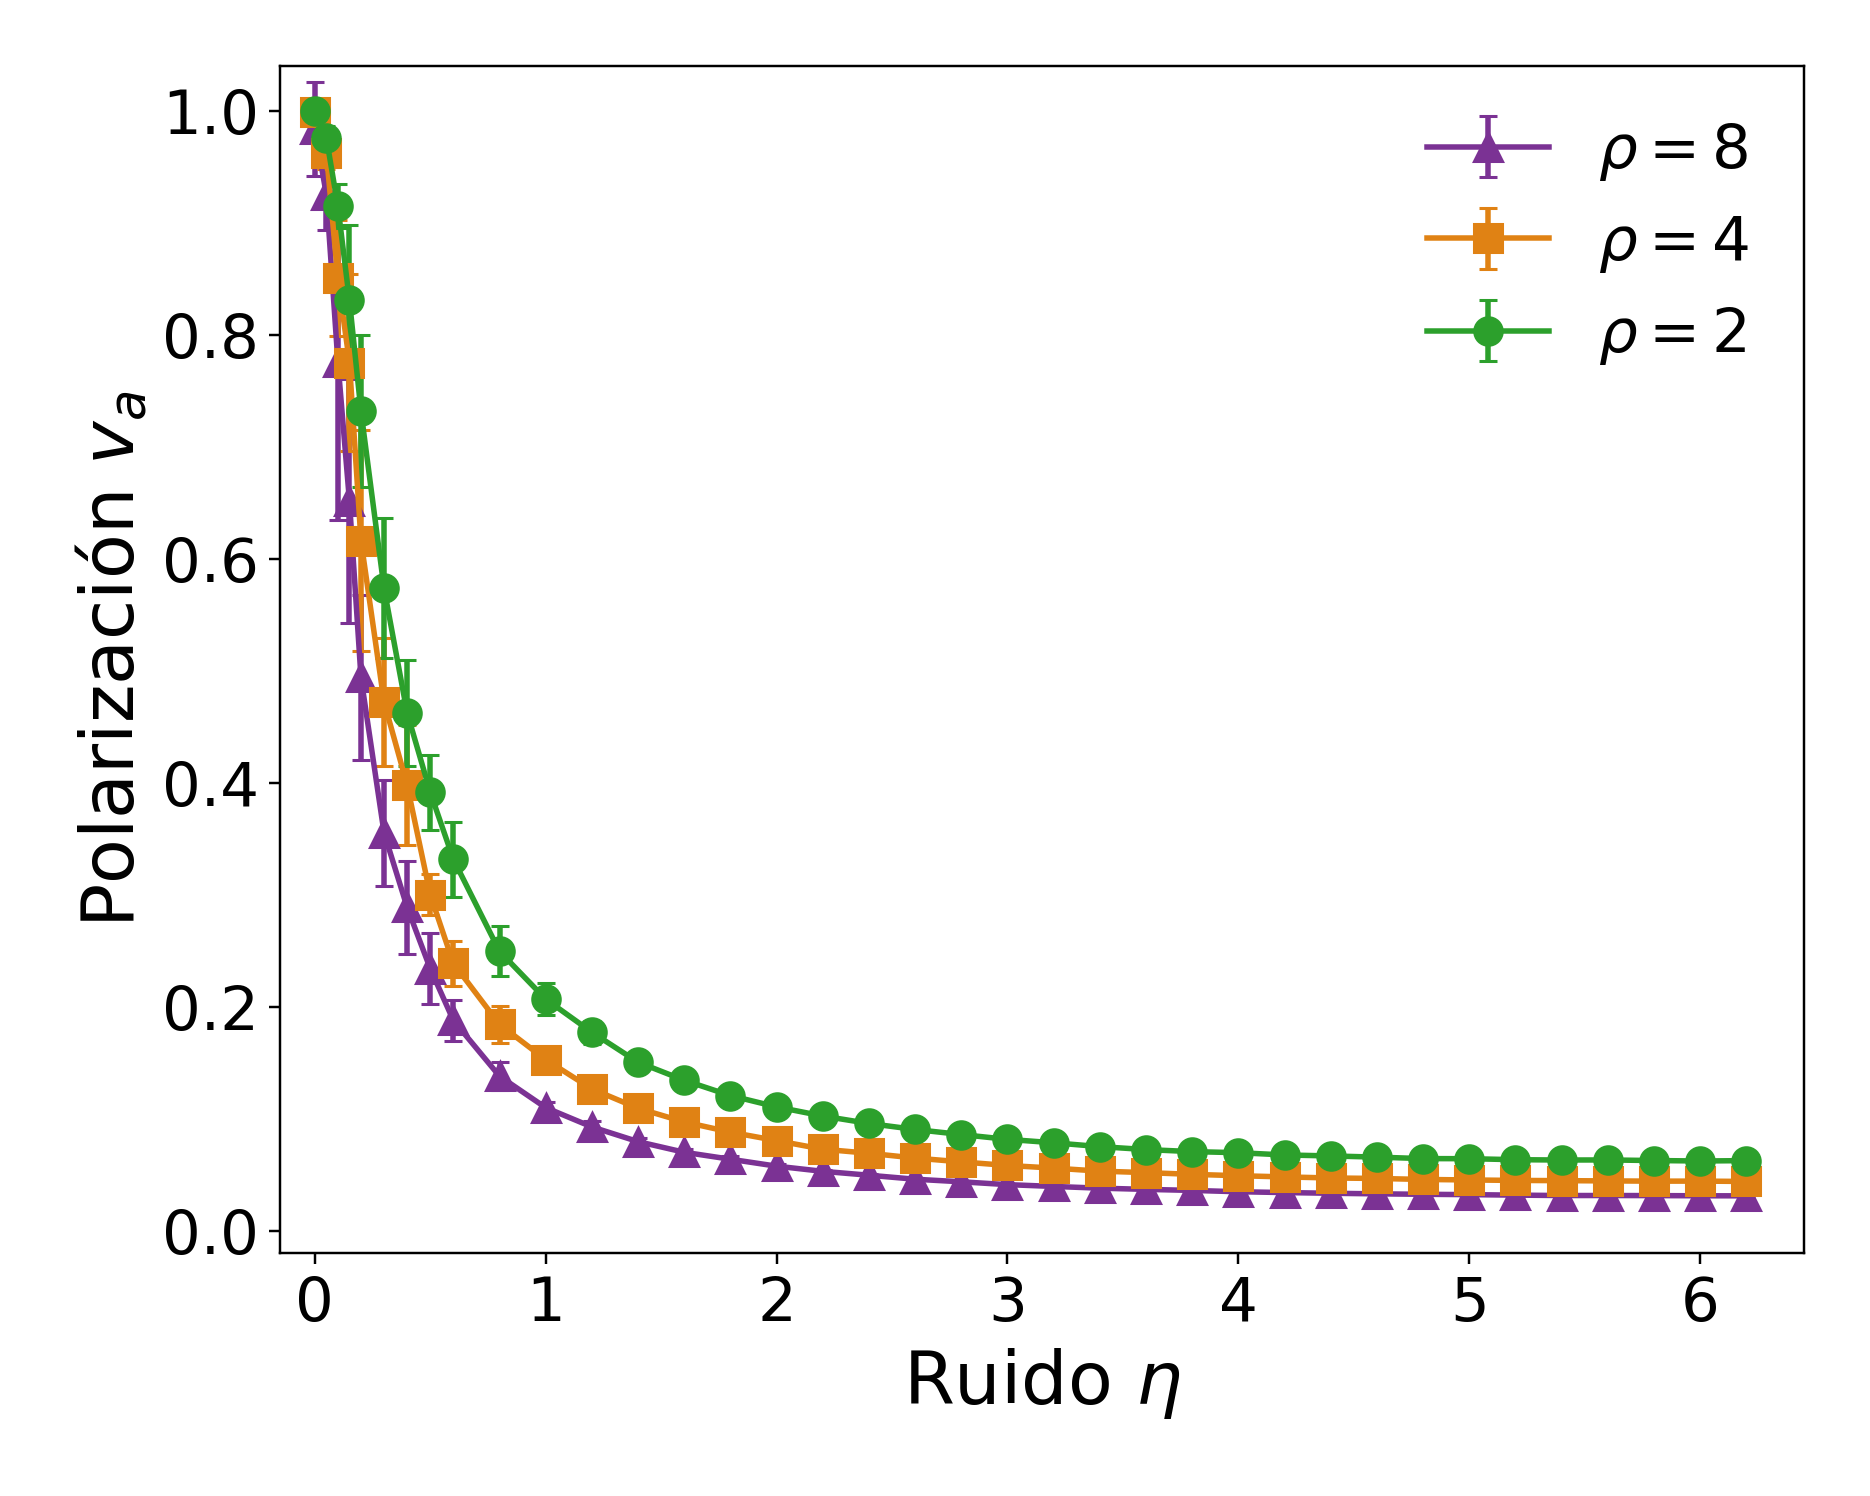
\includegraphics[width=0.85\linewidth]{figs/image6.png}
\caption{Polarización estacionaria en función del ruido para el modelo de votante y $\rho = 2$, $4$ y $8$. Cada punto se calculó a partir de $20$ realizaciones independientes; las barras indican desvío estándar entre realizaciones.}
\label{fig:6}
\end{figure}

\subsection{Comparación entre modelos}

La Fig.~\ref{fig:7} superpone las curvas de ambos modelos para las tres densidades. El resultado principal es que el modelo de votante pierde polarización a valores de ruido mucho menores que el modelo de Vicsek. En Vicsek, el promedio vectorial de las orientaciones vecinas amortigua las perturbaciones angulares y permite sostener el orden colectivo hasta ruidos más altos. En el votante, una orientación individual se propaga por copia, de modo que el ruido introducido en cada actualización no se promedia sobre el vecindario.

La dependencia con la densidad también difiere entre ambos modelos. En Vicsek, las curvas se desplazan hacia valores mayores de $v_a$ al aumentar $\rho$ en el régimen donde existe orden. En el votante, el ordenamiento observado es el opuesto: a igual $\eta$, las curvas de mayor $\rho$ se ubican generalmente por debajo. En conjunto, los resultados muestran que ambos mecanismos pueden generar orden direccional a ruido bajo, pero que el promedio vectorial de Vicsek es más robusto frente al ruido que la copia aleatoria propia del modelo de votante.

\begin{figure}[H]
\centering
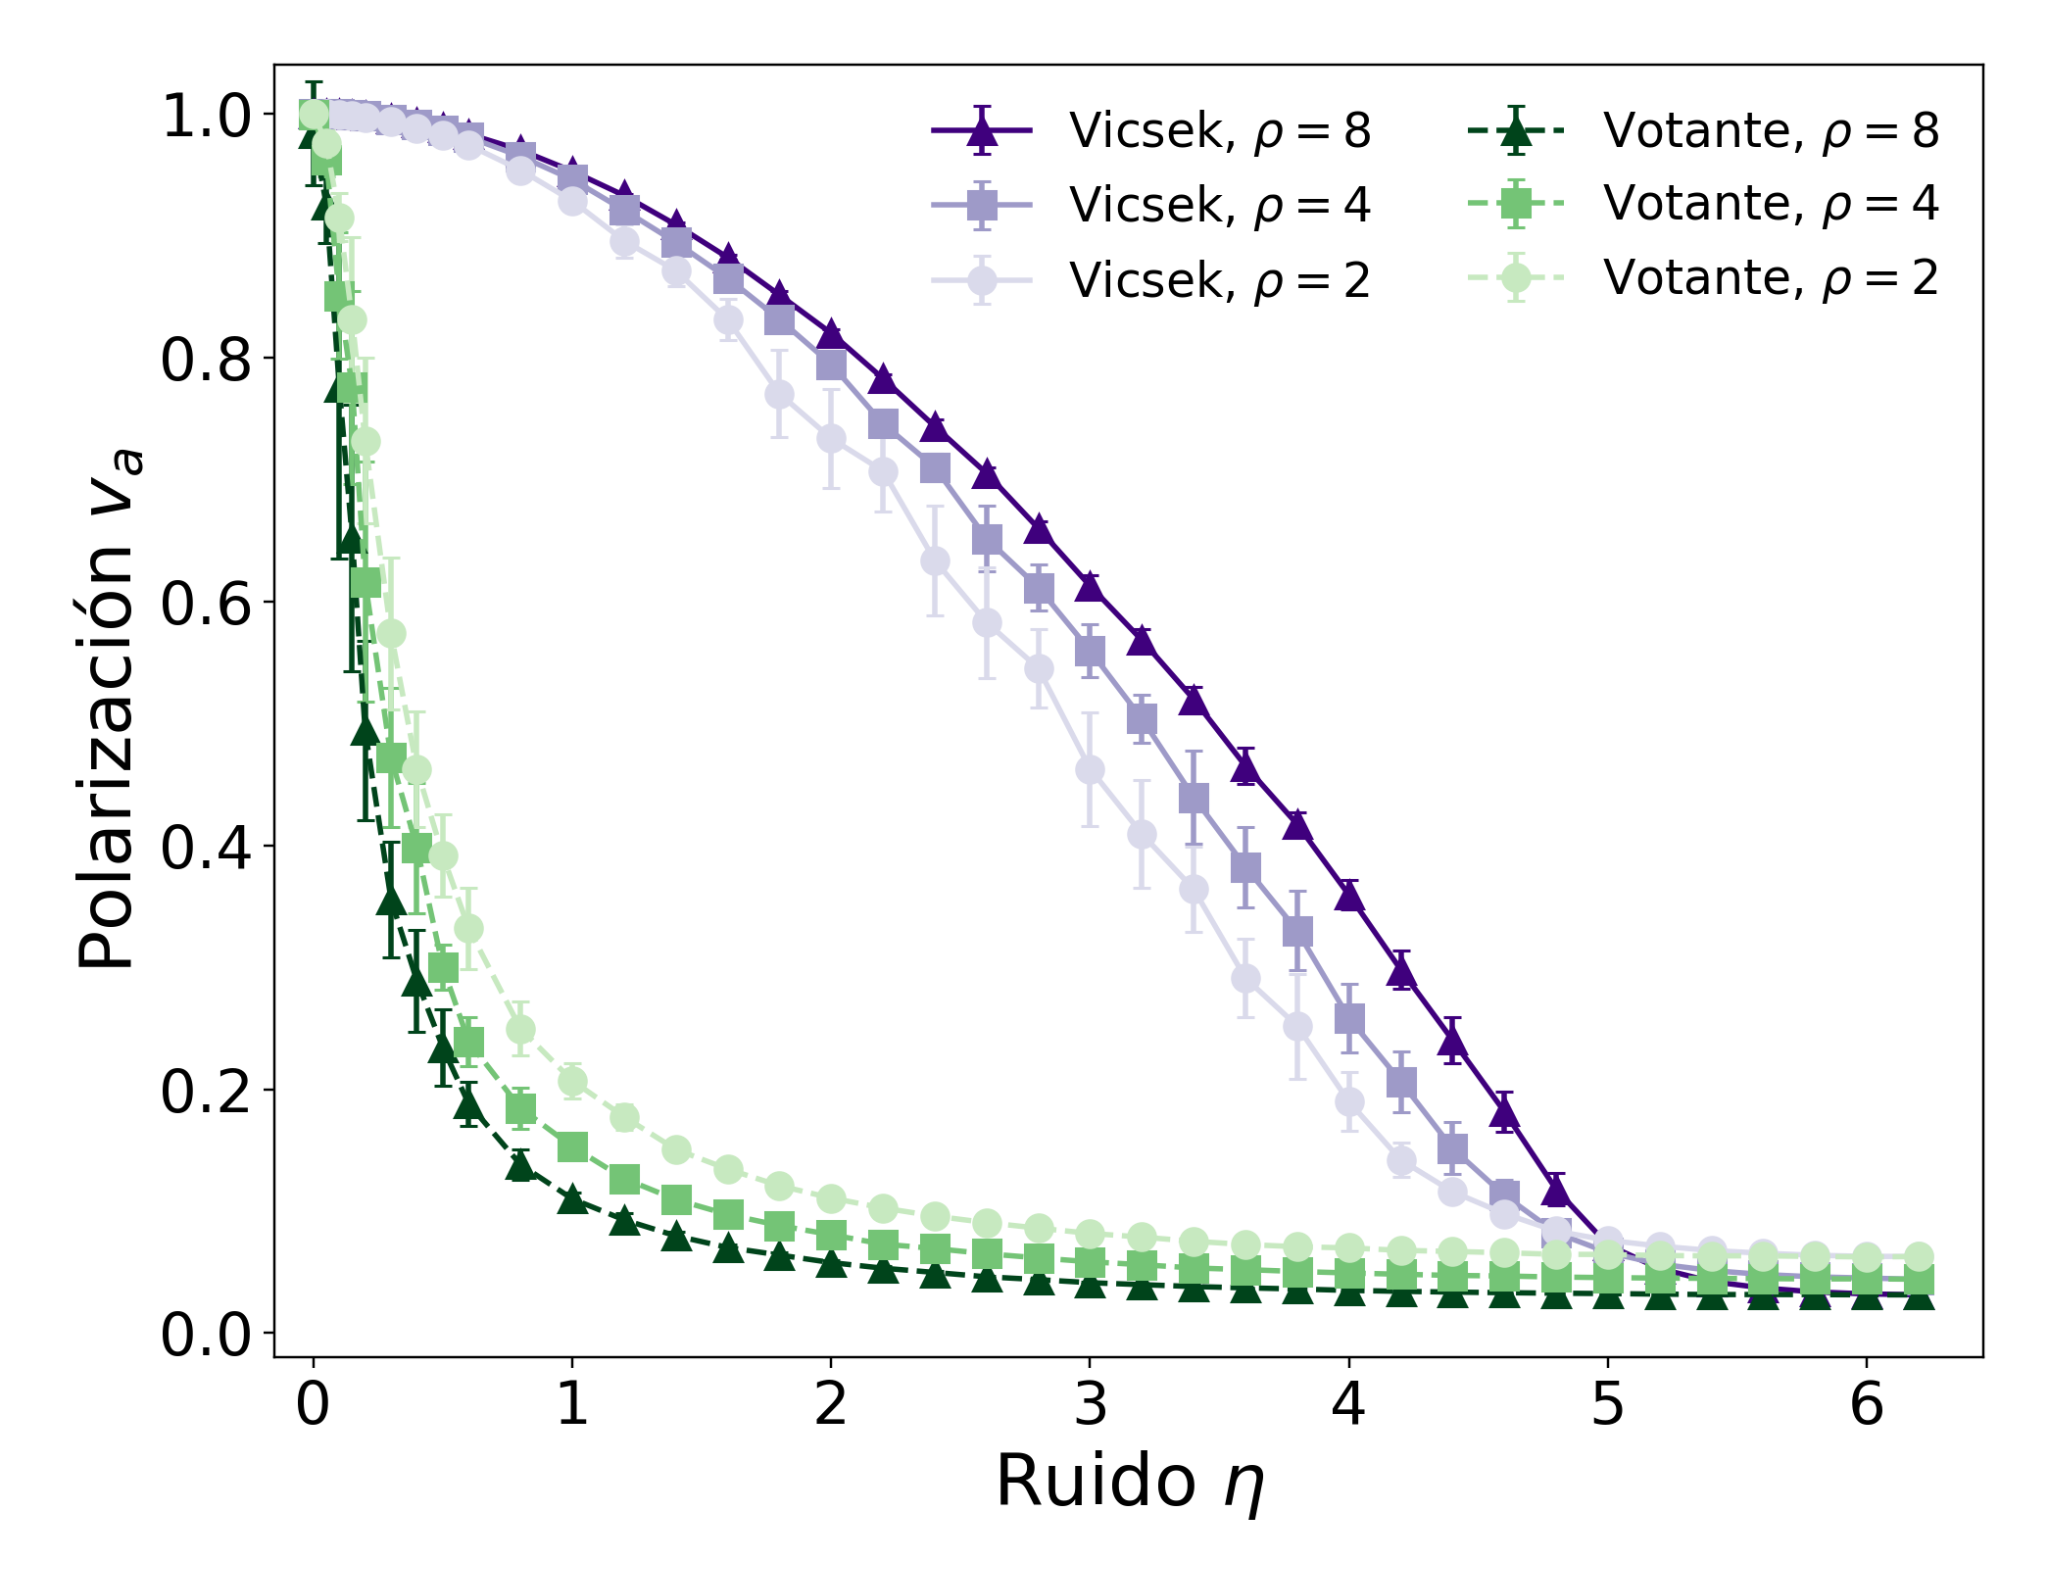
\includegraphics[width=0.85\linewidth]{figs/image7.png}
\caption{Comparación de la polarización estacionaria de Vicsek y votante para $\rho = 2$, $4$ y $8$. Las curvas violetas continuas corresponden a Vicsek y las verdes punteadas al votante; los marcadores distinguen las densidades. Los puntos y barras representan promedios y desvíos estándar sobre $20$ realizaciones independientes.}
\label{fig:7}
\end{figure}

% ---------------------------------------------------------------------
\section{Clusters y relación entre $S$ y $v_a$}
\label{sec:clusters}
% ---------------------------------------------------------------------

El segundo observable analizado fue la fracción de partículas contenida en la componente conexa más grande de la red de vecinos,

\begin{equation}
S(t) = \frac{n_{\max}(t)}{N},
\label{eq:S}
\end{equation}

donde $n_{\max}(t)$ se construye con el mismo criterio de vecindad de la Ec.~\ref{eq:vecindad}.

Las Figs.~\ref{fig:8} y~\ref{fig:9} muestran, a modo de ejemplo, la evolución temporal de $S$ para una única realización en $\rho = 1/\pi$ ($N=32$). En Vicsek ($\eta = 1$, $3$ y $5$) y en votante ($\eta = 0.05$, $0.3$ y $1$), $S$ fluctúa con amplitud grande alrededor de un nivel medio que decrece con $\eta$, sin estabilizarse en un valor fijo. Esta variabilidad es mayor que la observada en $v_a$ para la misma densidad y responde al tamaño chico del sistema: con pocas partículas, cada cambio de vecindad mueve a $S$ en saltos discretos apreciables.

\begin{figure}[H]
\centering
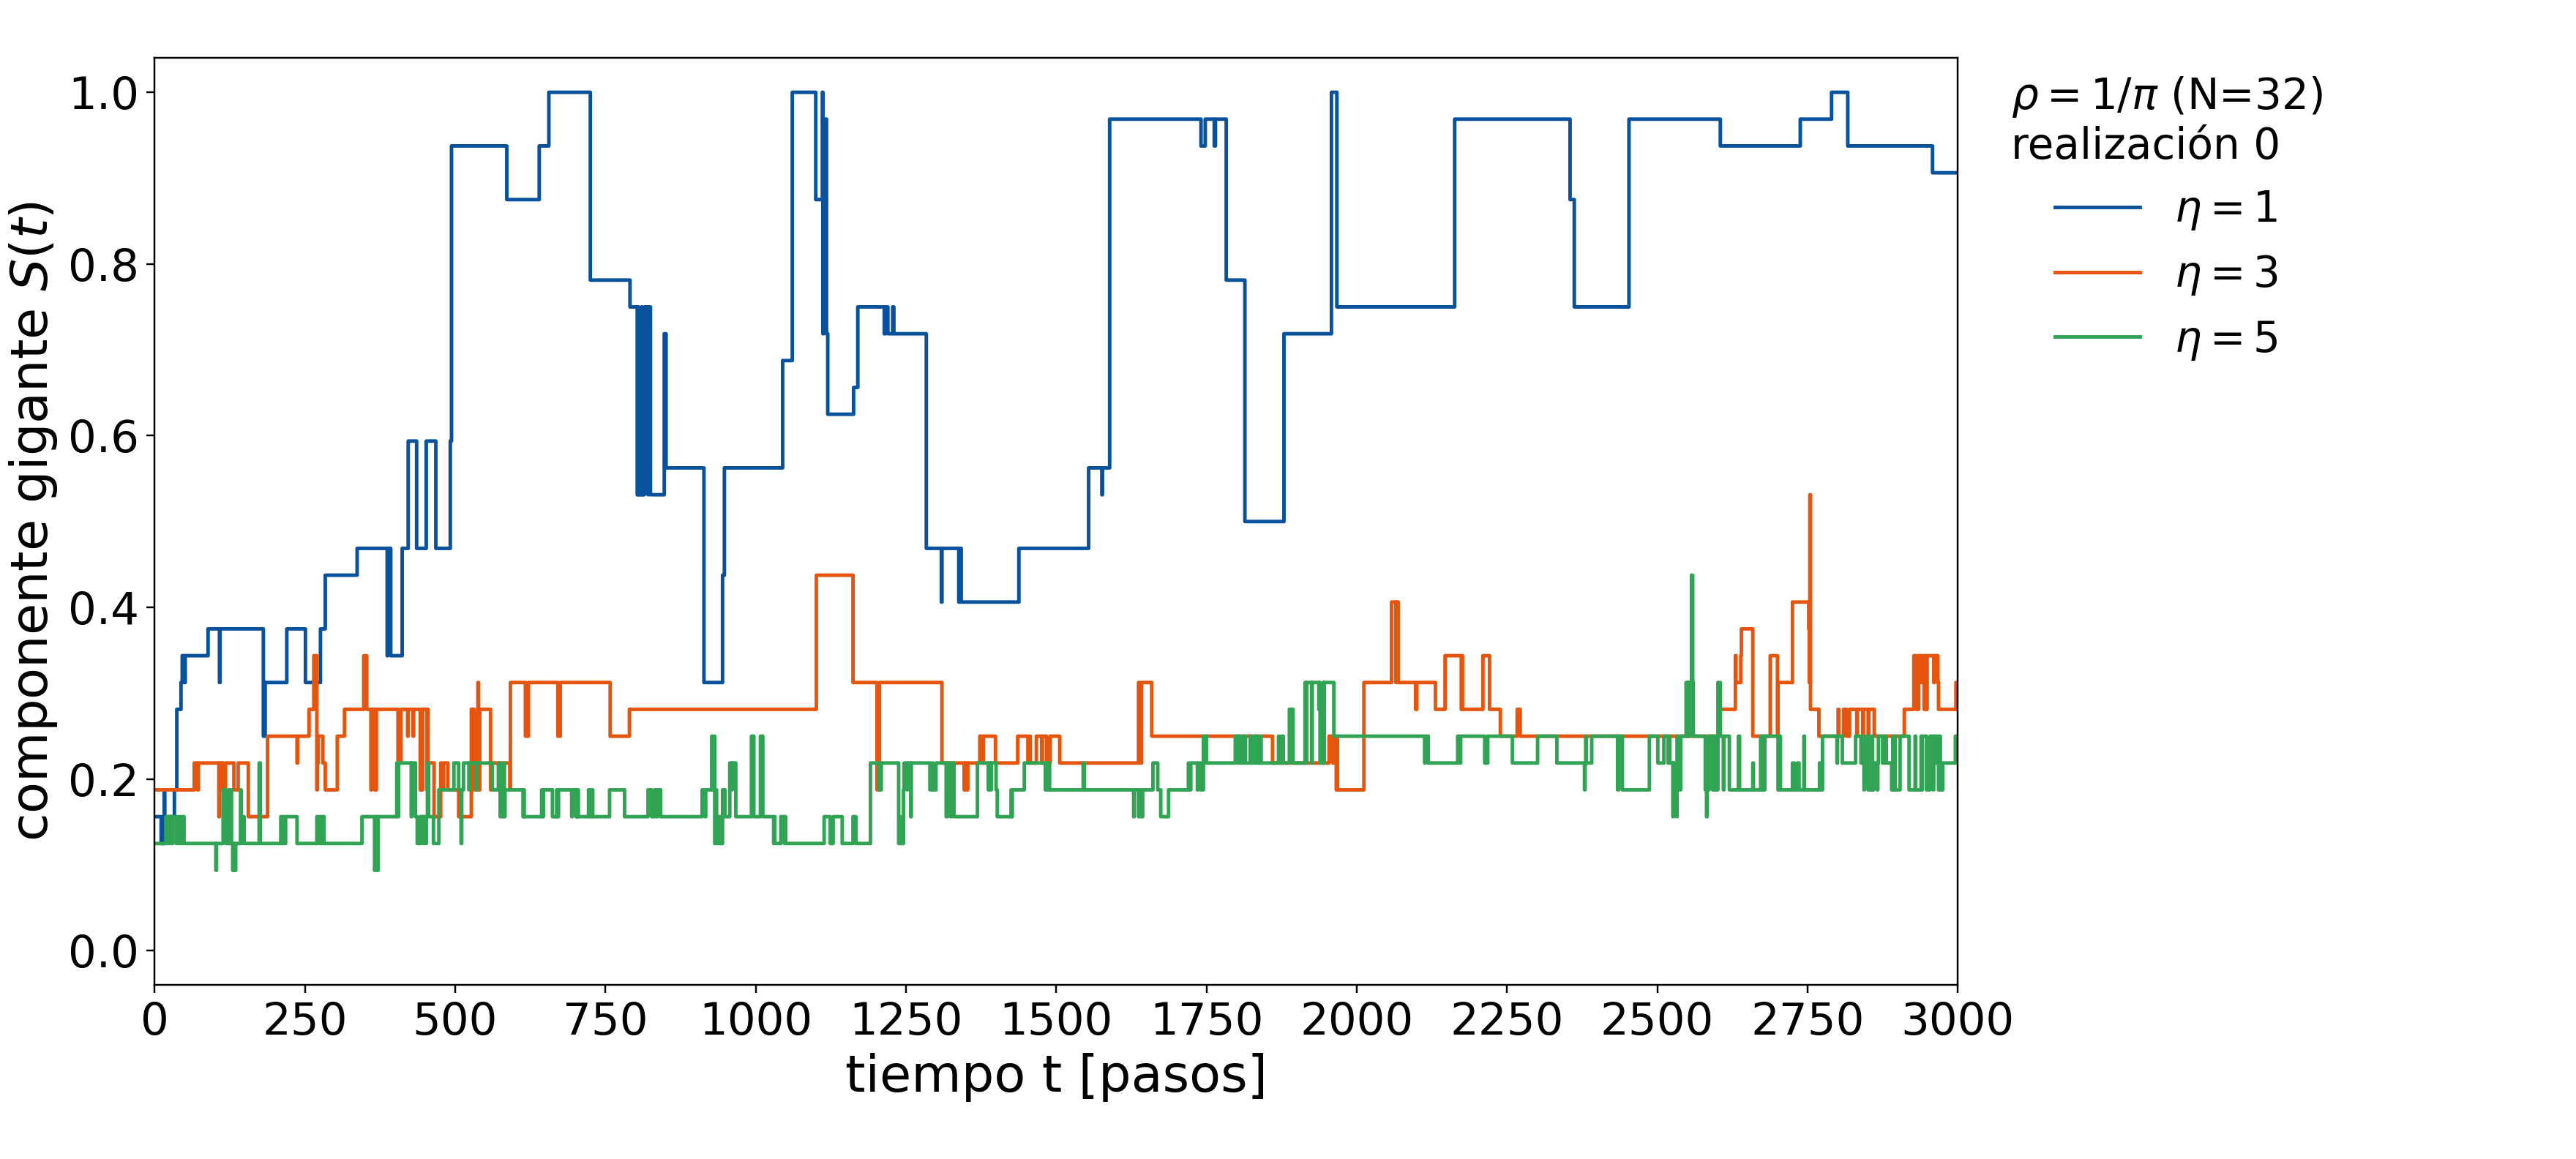
\includegraphics[width=0.85\linewidth]{figs/image8.png}
\caption{Evolución temporal de $S$ en el modelo de Vicsek para $\rho = 1/\pi$ ($N=32$), una realización. $\eta = 1$, $3$ y $5$.}
\label{fig:8}
\end{figure}

\begin{figure}[H]
\centering
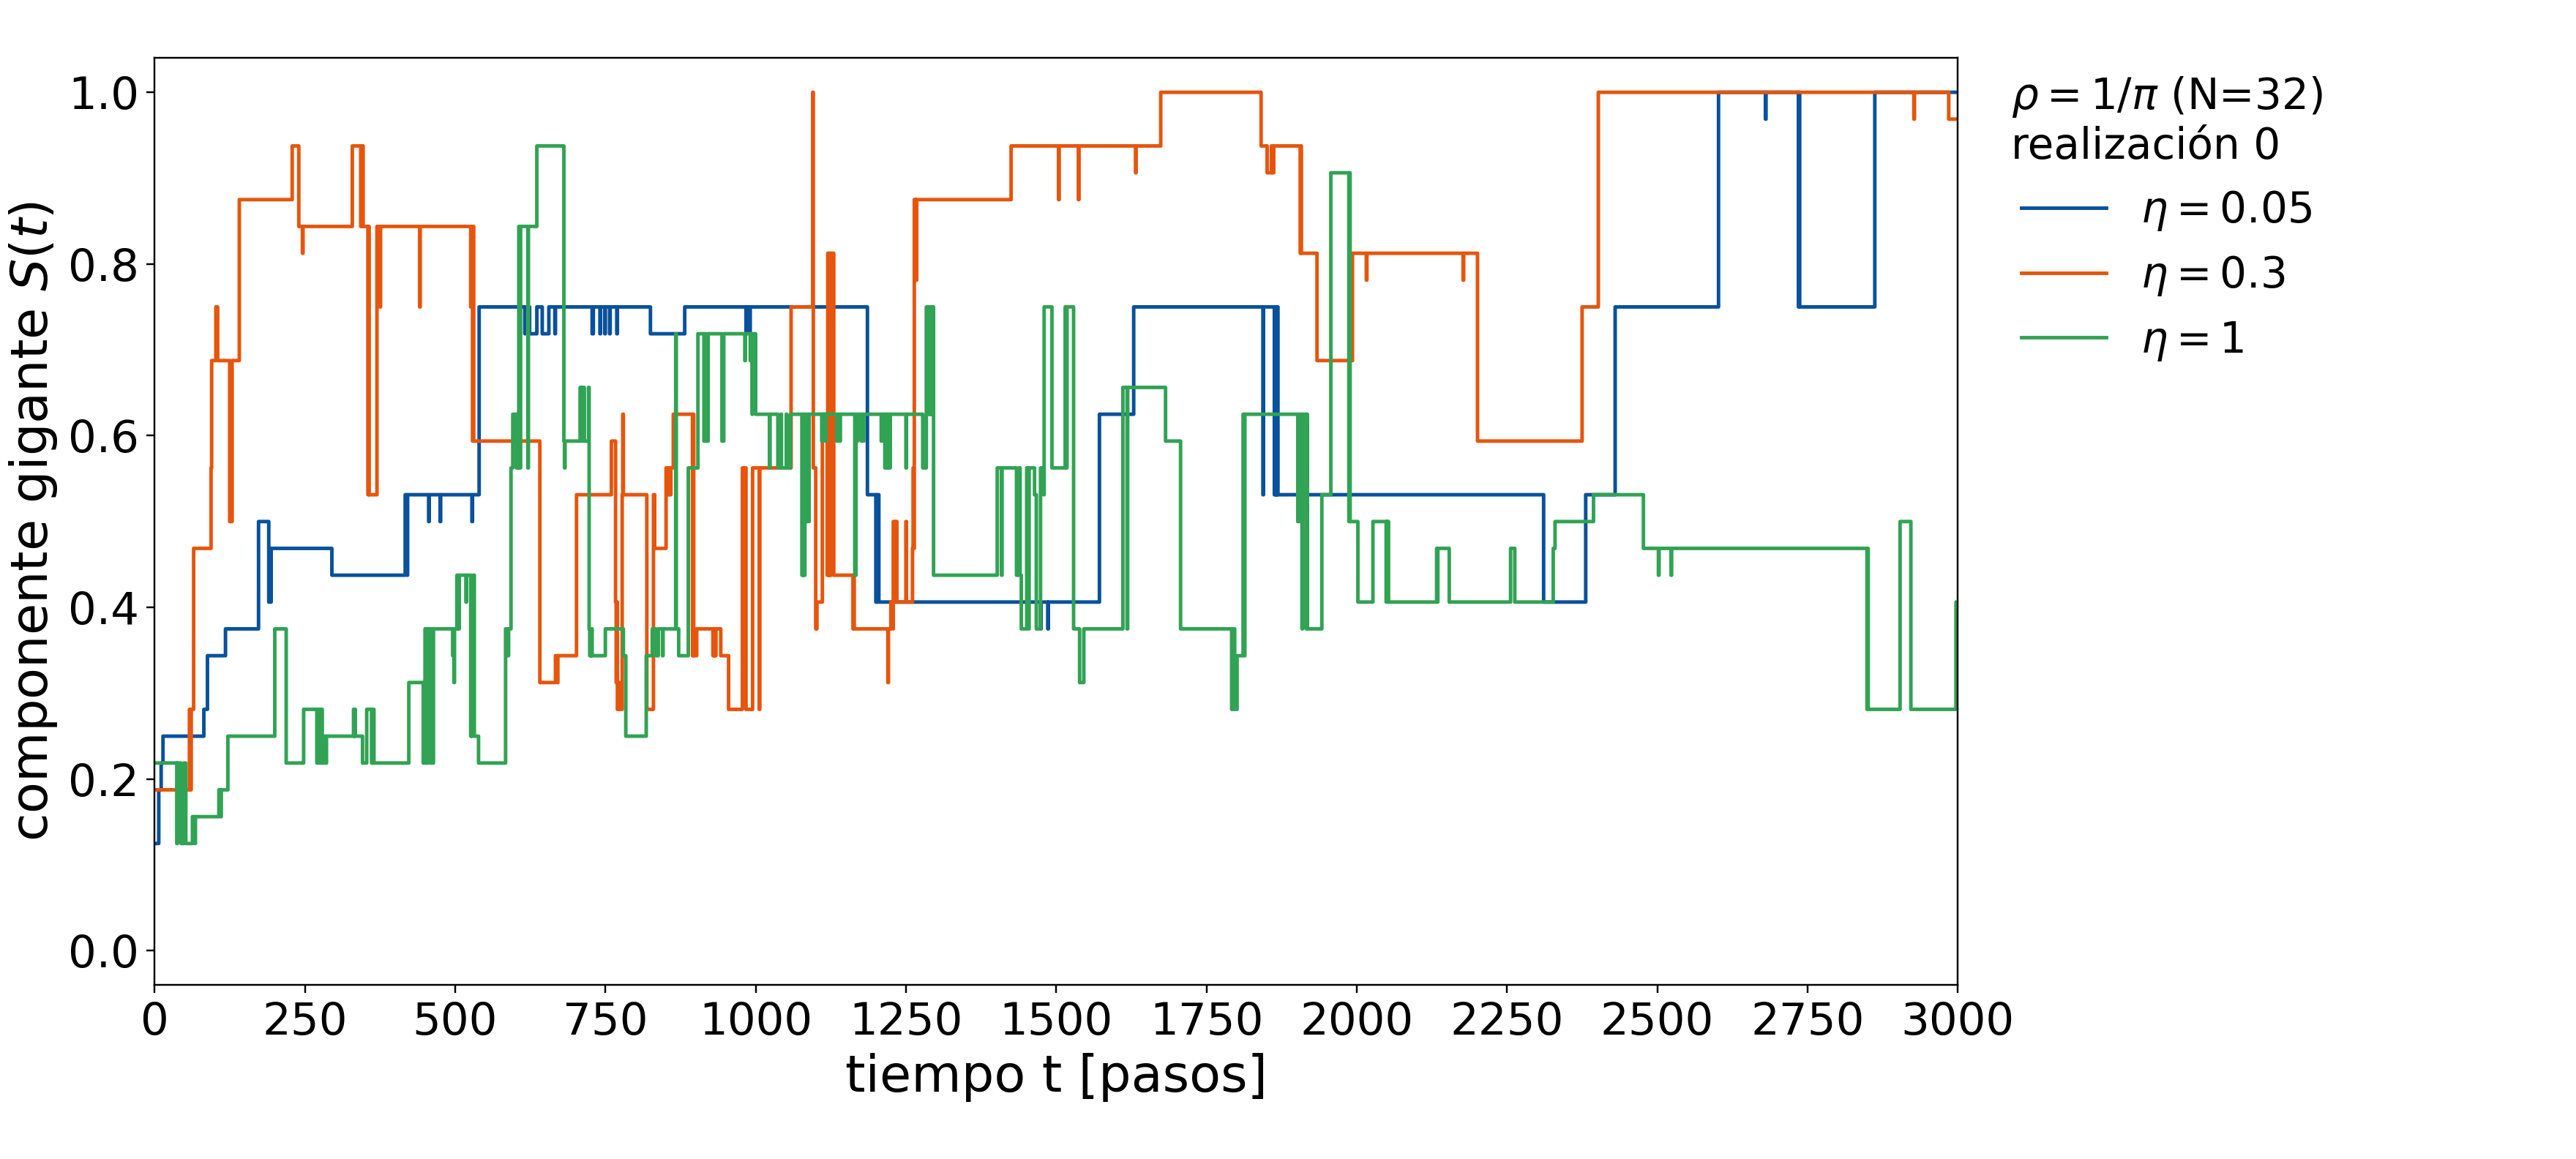
\includegraphics[width=0.85\linewidth]{figs/image9.png}
\caption{Evolución temporal de $S$ en el modelo de votante para $\rho = 1/\pi$ ($N=32$), una realización. $\eta = 0.05$, $0.3$ y $1$.}
\label{fig:9}
\end{figure}

Las Figs.~\ref{fig:10} y~\ref{fig:11} muestran el promedio estacionario de $S$ en función de $\eta$ para las seis densidades estudiadas: $\rho = 2$, $4$ y $8$ ($N=200,400,800$) y las tres densidades bajas del estudio de clusters, $\rho_{\text{nominal}} = 1/\pi$, $1/(2\pi)$ y $1/(3\pi)$ ($N=32,16,11$ por redondeo al entero más cercano, $\rho_{\text{efectiva}}=0.32,0.16,0.11$). En ambos modelos, $\rho = 2$, $4$ y $8$ mantienen $S$ cercano a $1$ en todo el barrido, mientras que las tres densidades bajas caen de forma marcada y continua con $\eta$, desde valores iniciales cercanos a $0.9$ hasta aproximadamente $0.15$--$0.2$ en $\eta$ alto. Esto es consistente con el número medio de vecinos externos de cada densidad: del orden de $6$ a $25$ en $\rho=2,4,8$, frente a $1$, $0.5$ y $0.33$ en las densidades bajas, donde la red queda mucho más cerca del límite de conectividad.

\begin{figure}[H]
\centering
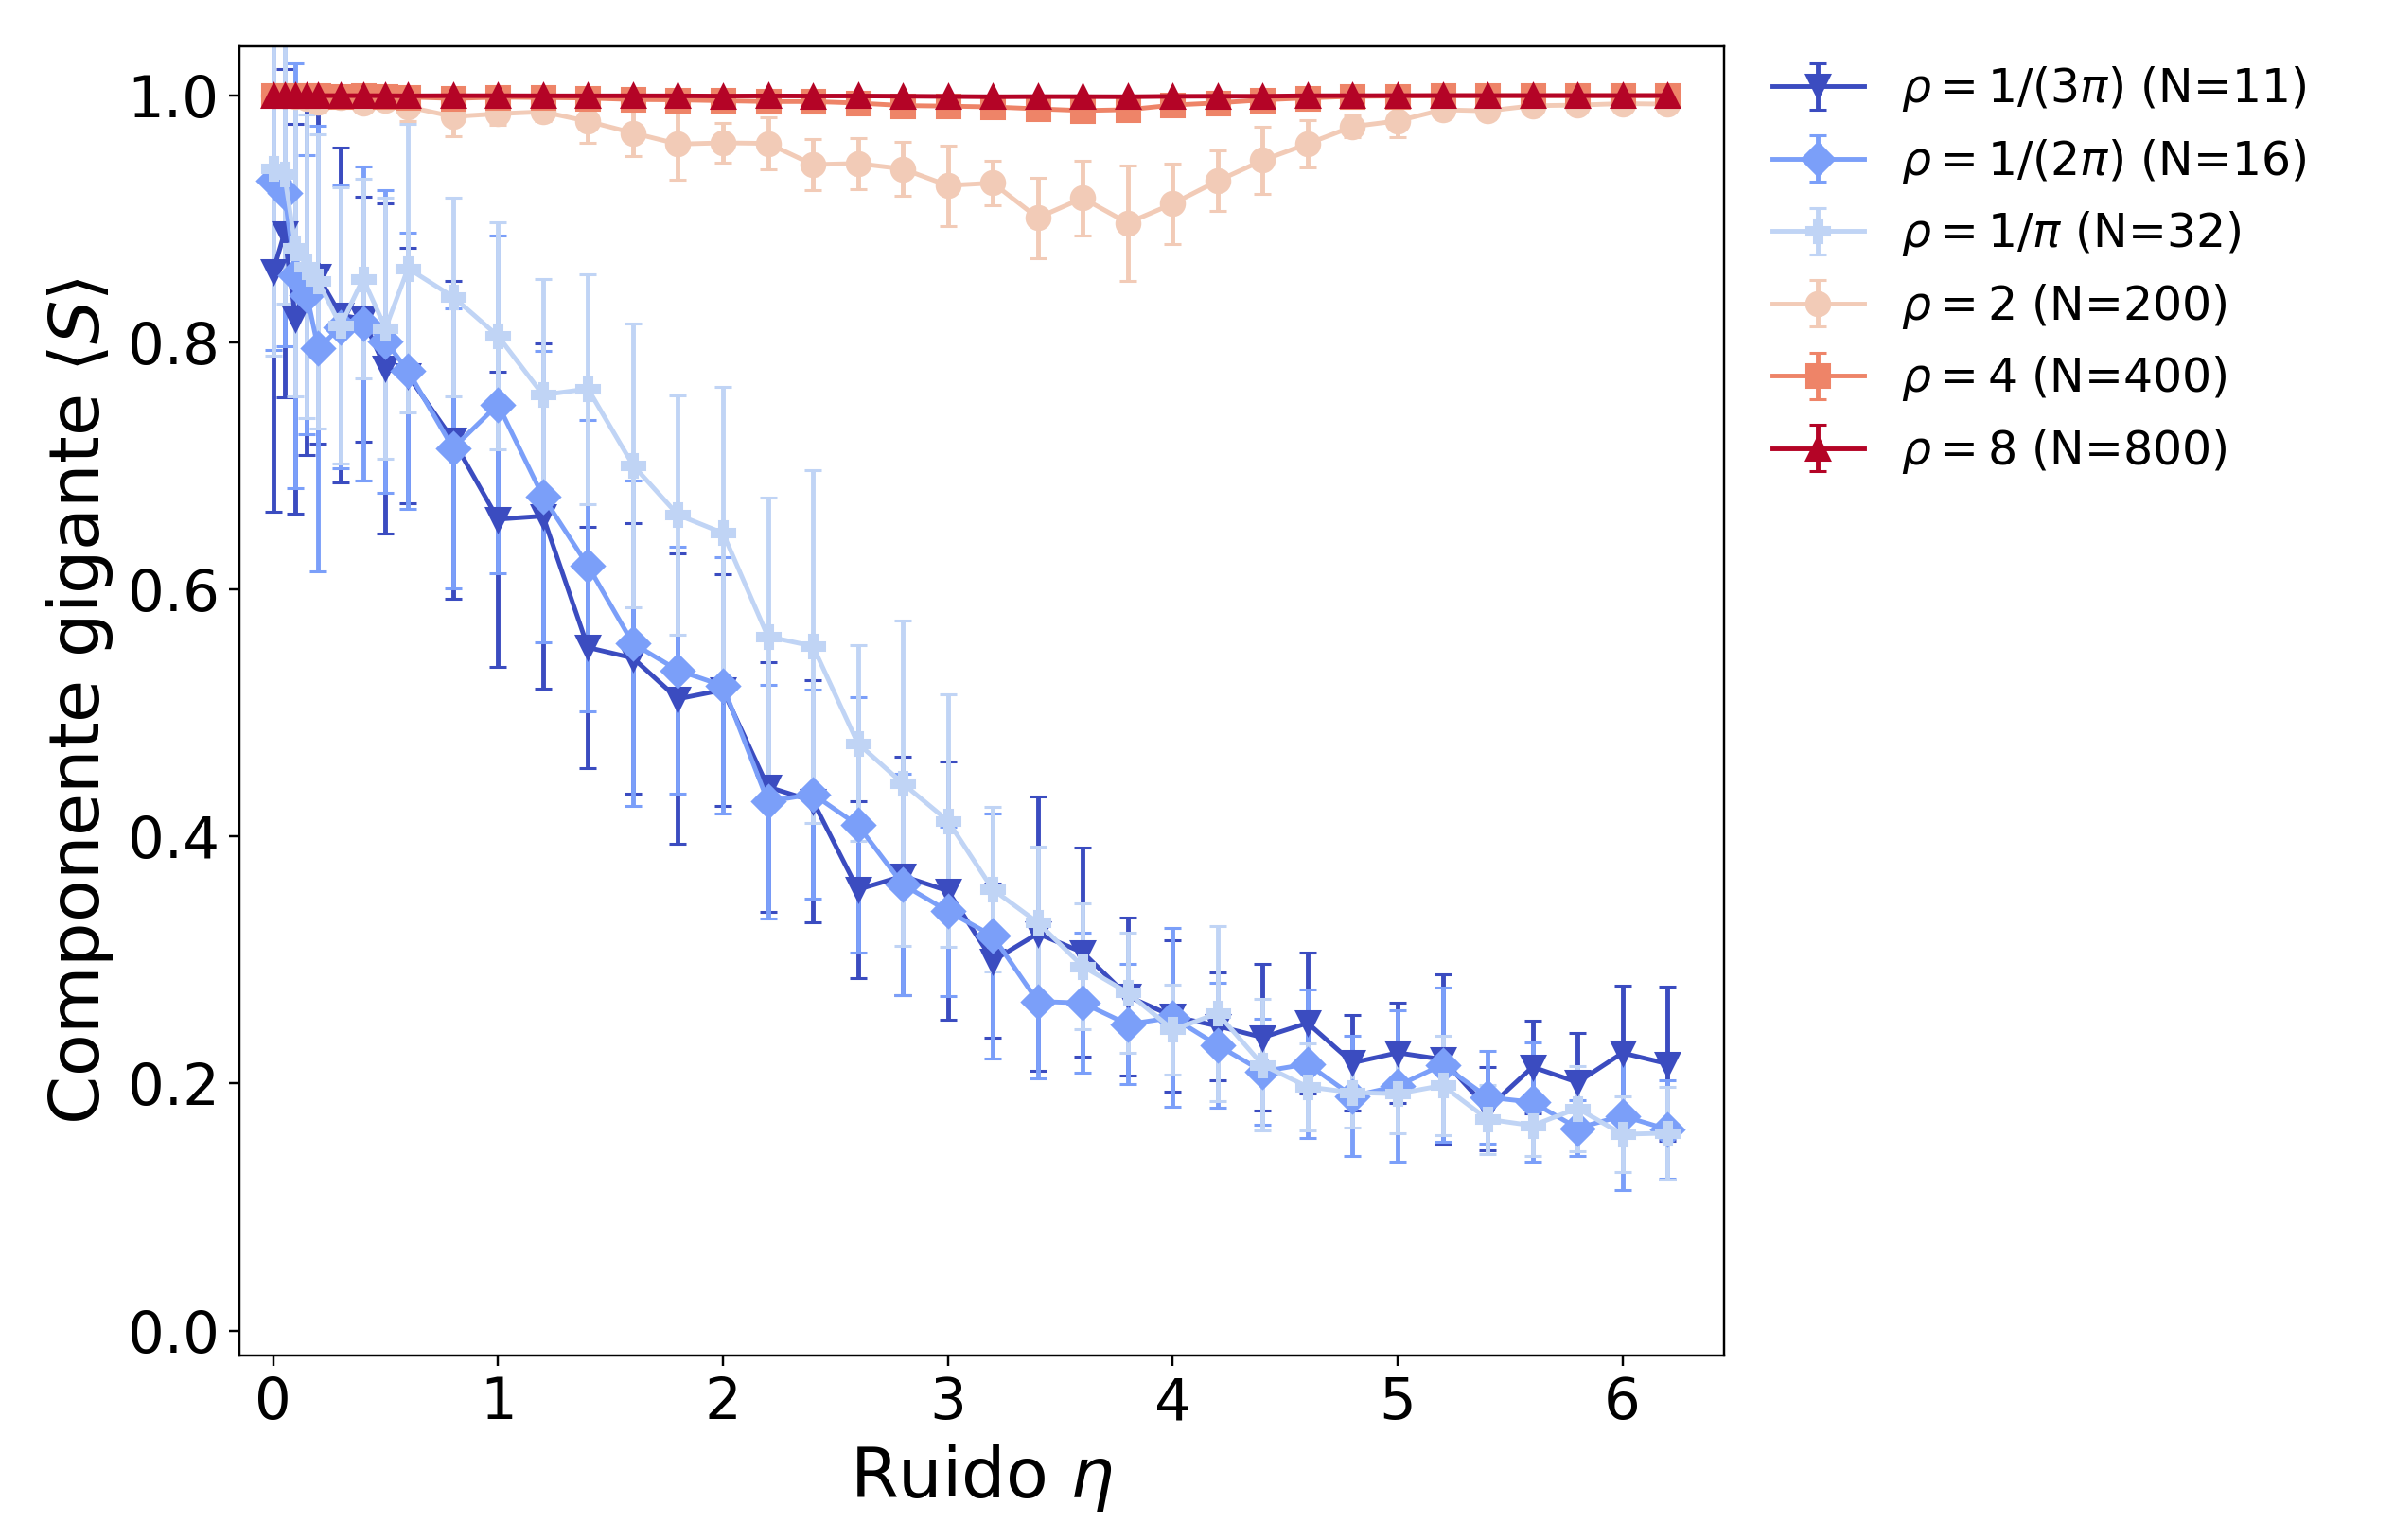
\includegraphics[width=0.85\linewidth]{figs/image10.png}
\caption{Componente gigante estacionaria en función del ruido para el modelo de Vicsek, seis densidades ($\rho=1/(3\pi),1/(2\pi),1/\pi,2,4,8$).}
\label{fig:10}
\end{figure}

\begin{figure}[H]
\centering
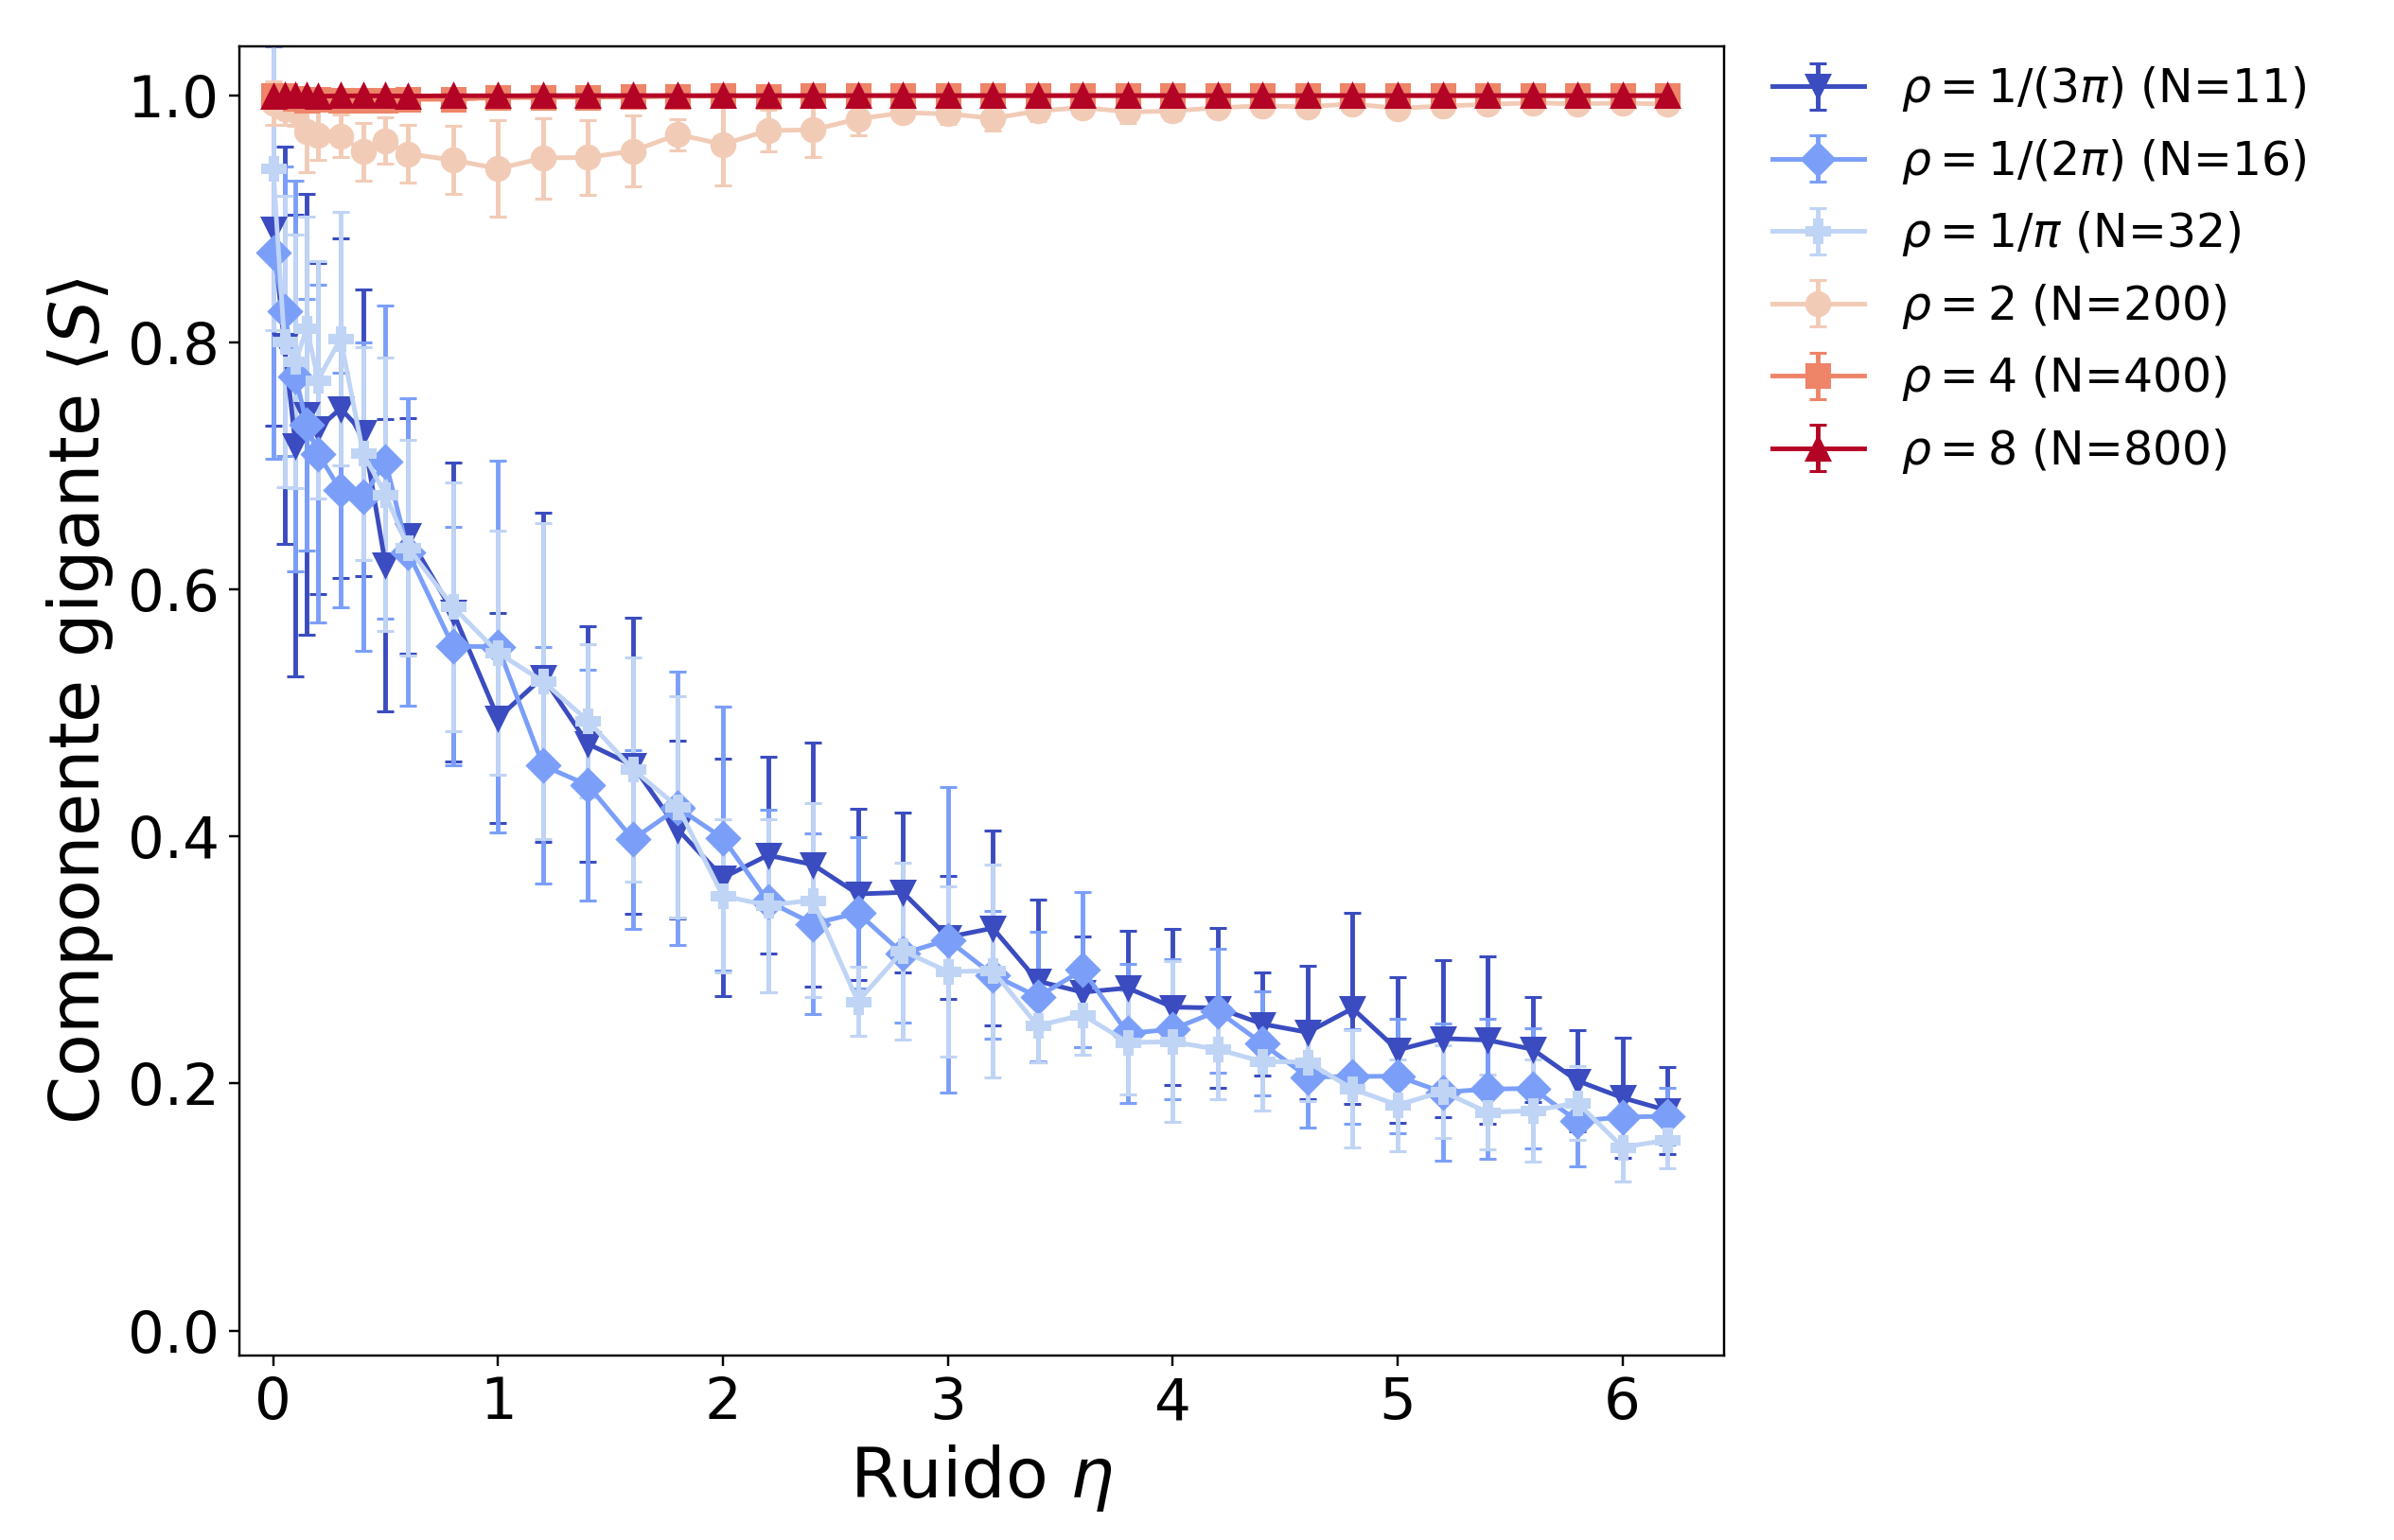
\includegraphics[width=0.85\linewidth]{figs/image11.png}
\caption{Componente gigante estacionaria en función del ruido para el modelo de votante, seis densidades ($\rho=1/(3\pi),1/(2\pi),1/\pi,2,4,8$).}
\label{fig:11}
\end{figure}

La Fig.~\ref{fig:12} compara ambos modelos restringida a las tres densidades bajas, donde la diferencia entre reglas es visible. Para $\eta$ entre aproximadamente $1$ y $3$, el votante presenta valores de $S$ sistemáticamente menores que Vicsek a igual densidad; ambos modelos convergen a valores similares para $\eta \gtrsim 4$. Una explicación posible es que, con pocos vecinos disponibles, promediar toda la vecindad sostiene mejor la cohesión espacial que copiar a un único vecino; el estudio no aísla esta hipótesis de otras diferencias entre modelos.

\begin{figure}[H]
\centering
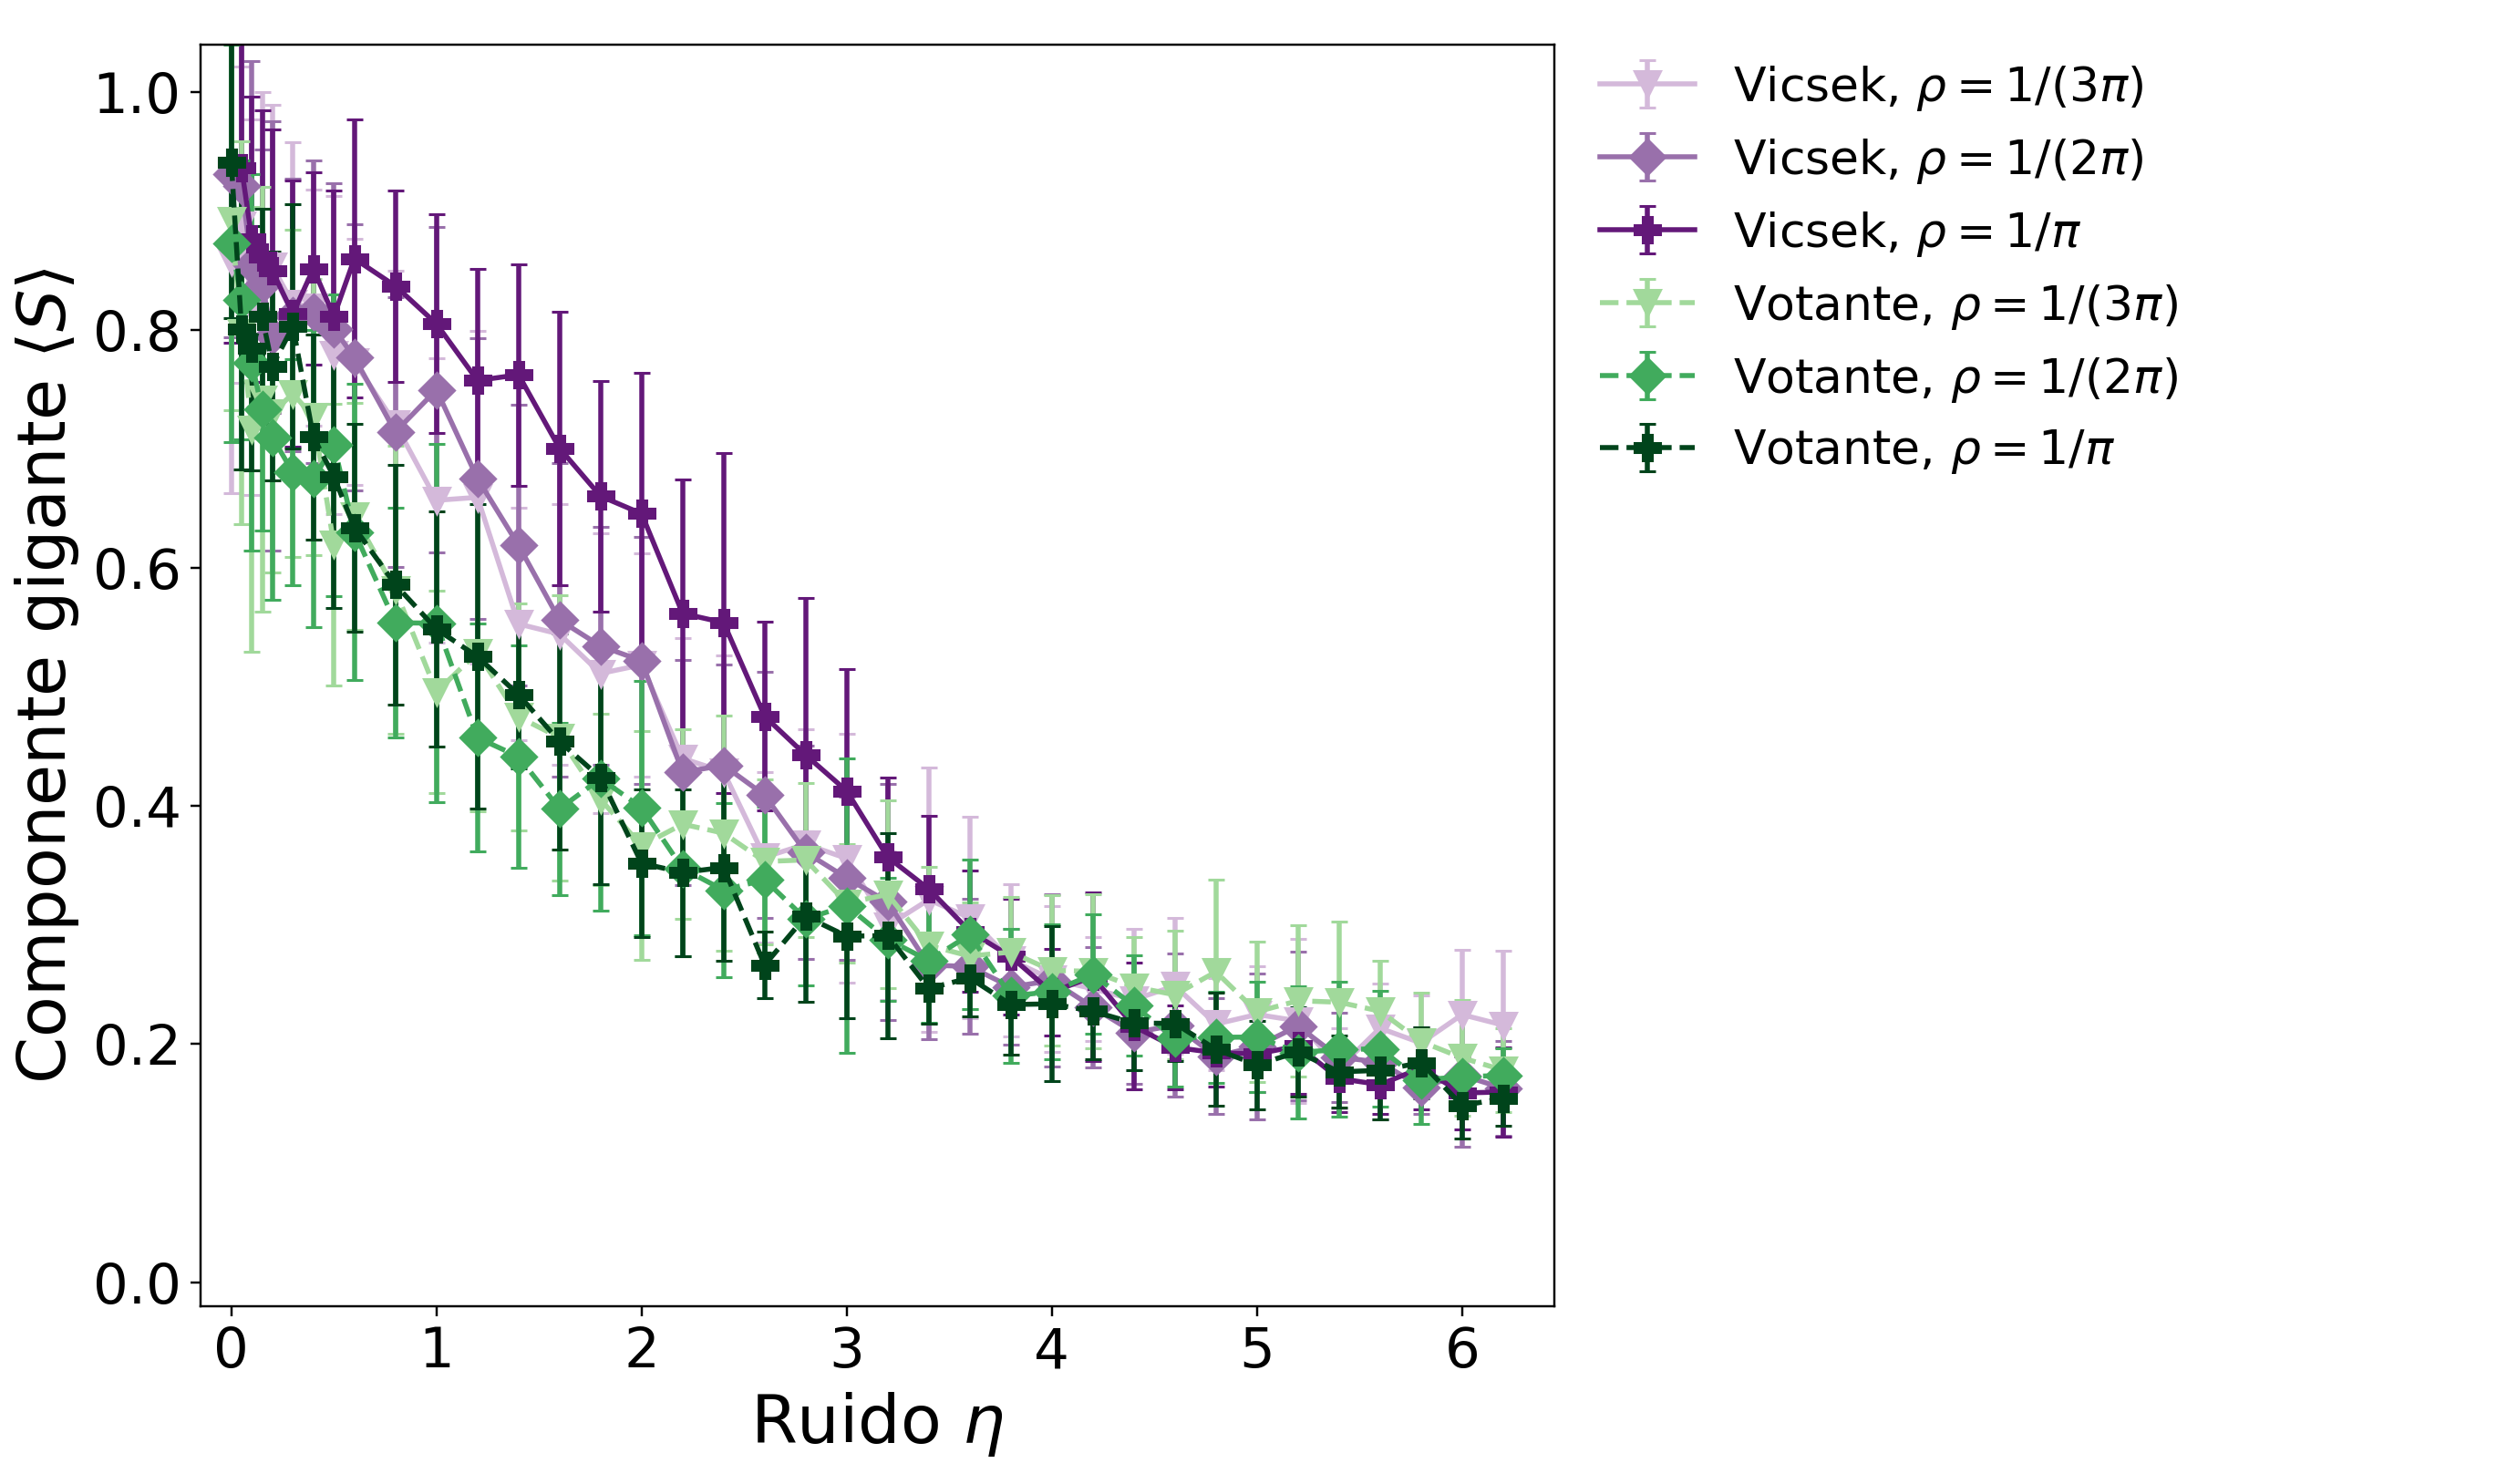
\includegraphics[width=0.85\linewidth]{figs/image12.png}
\caption{Componente gigante estacionaria en función del ruido, Vicsek y votante superpuestos, para las tres densidades bajas ($\rho=1/(3\pi),1/(2\pi),1/\pi$).}
\label{fig:12}
\end{figure}

Finalmente, la Fig.~\ref{fig:13} relaciona $v_a$ y $S$ para $\rho = 2$ junto con las tres densidades bajas, un punto por cada $\eta$ del barrido. En $\rho = 2$, $S$ permanece cercano a $1$ para casi cualquier valor de $v_a$: la nube resulta casi horizontal. En las tres densidades bajas, en cambio, $S$ y $v_a$ decrecen juntos de forma aproximadamente monótona, formando una tendencia creciente entre ambos observables. Esto indica que la relación entre conectividad espacial y orden direccional depende de la densidad: en $\rho=2$ son prácticamente independientes, mientras que en las densidades bajas, donde la red está cerca de su límite de conectividad, un menor orden direccional se asocia con una red más fragmentada.

\begin{figure}[H]
\centering
\begin{minipage}{0.48\linewidth}
\centering
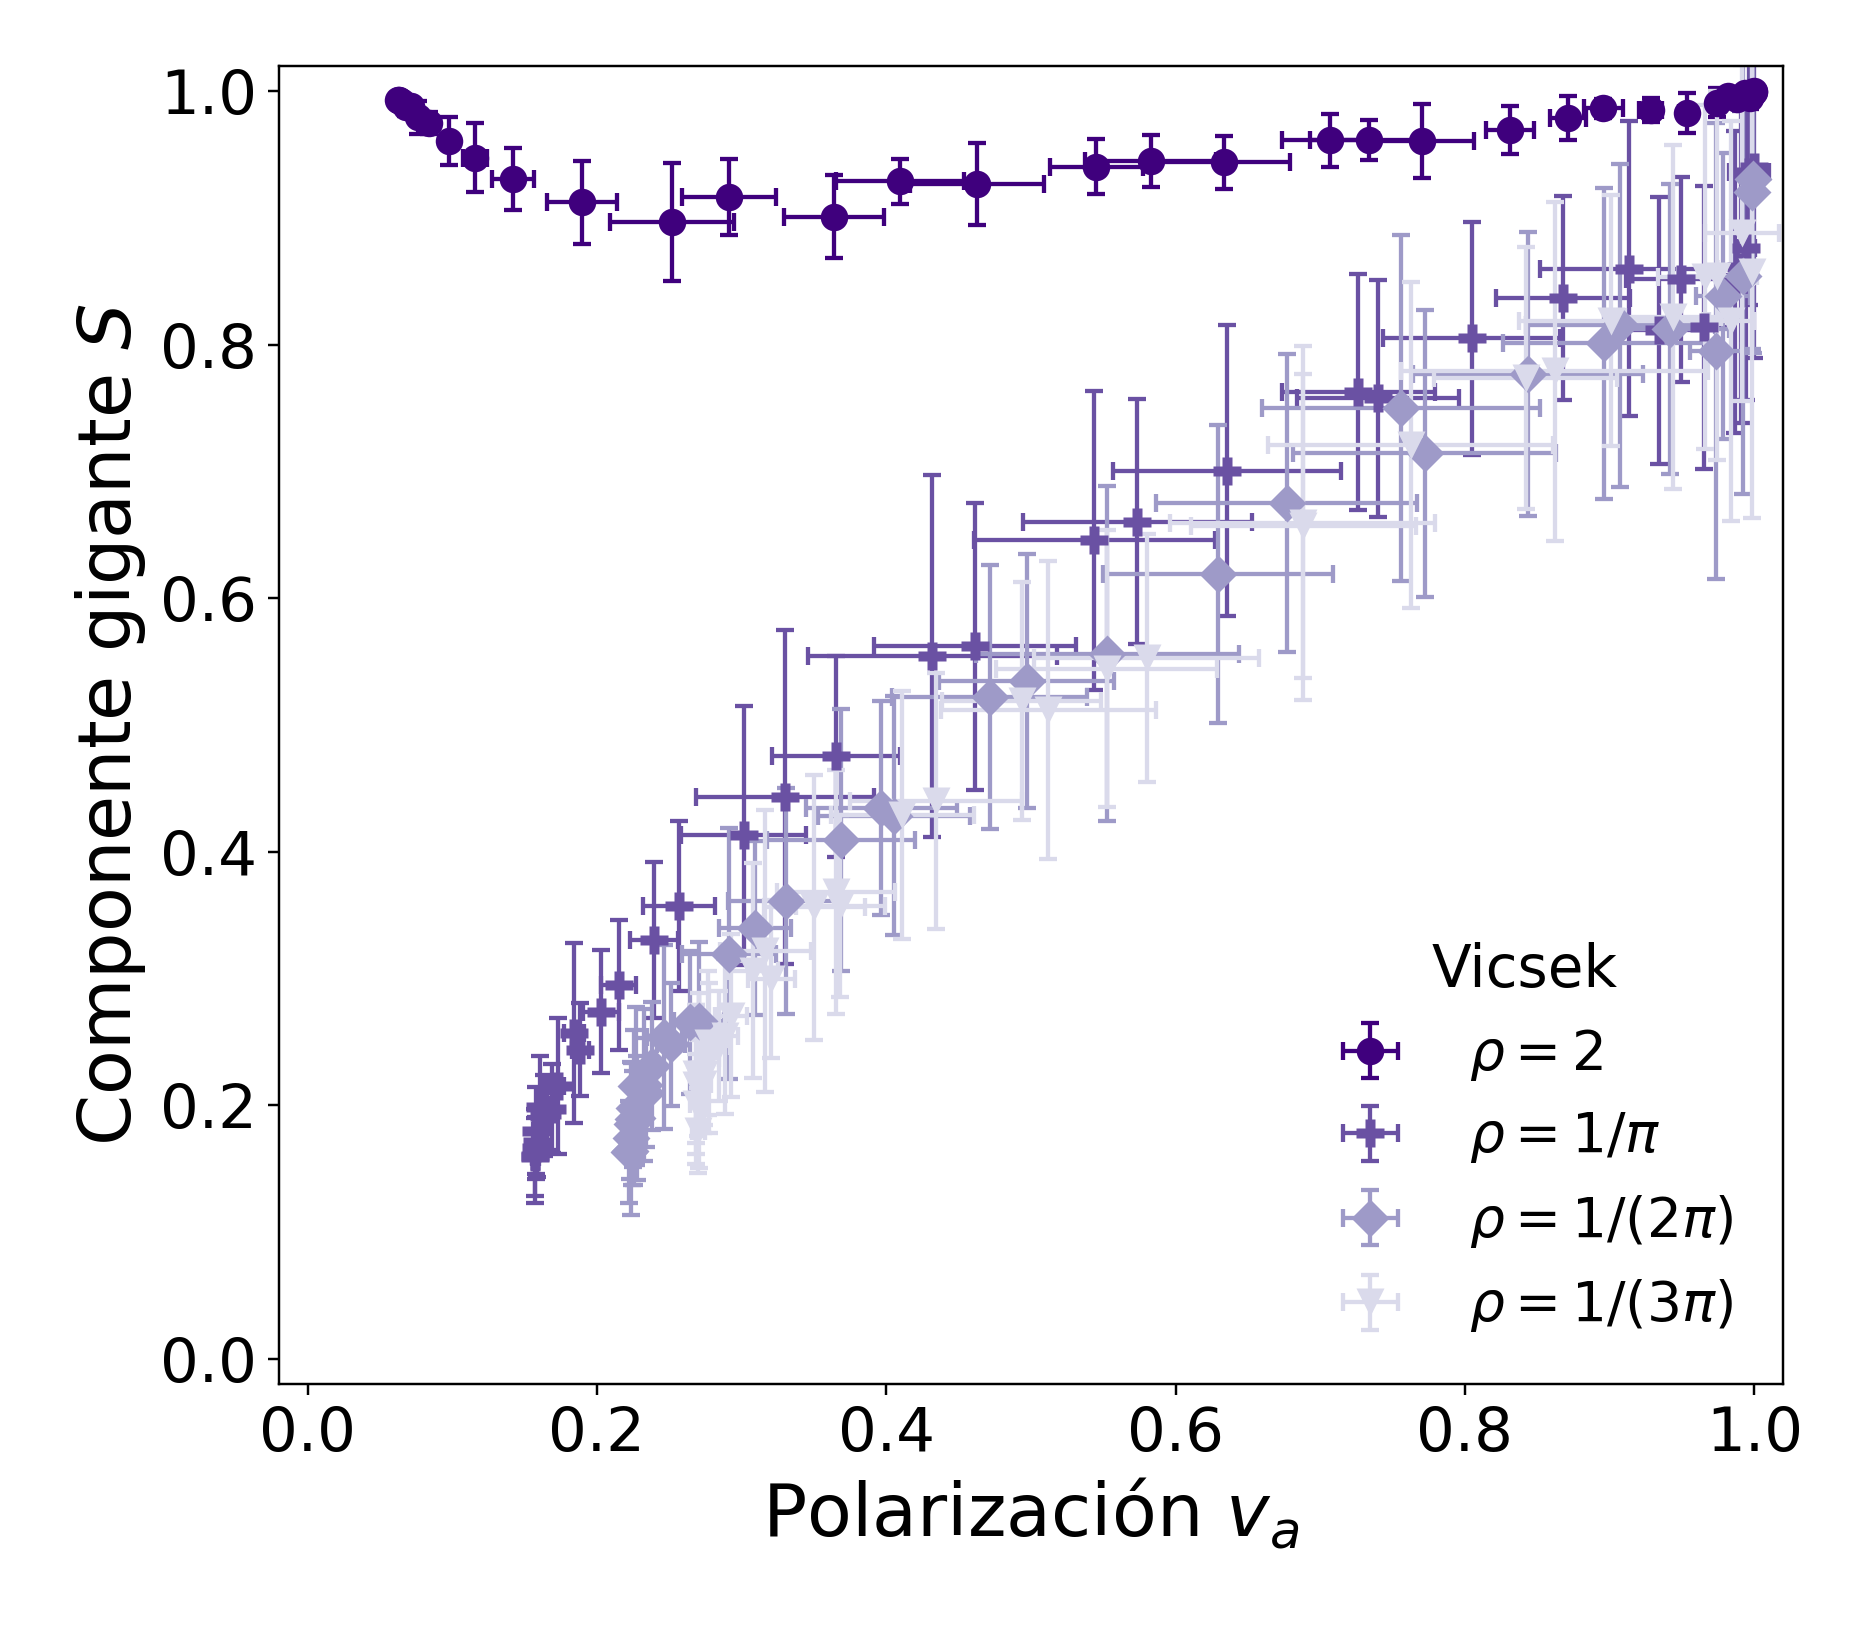
\includegraphics[width=\linewidth]{figs/image13a.png}
\end{minipage}
\hfill
\begin{minipage}{0.48\linewidth}
\centering
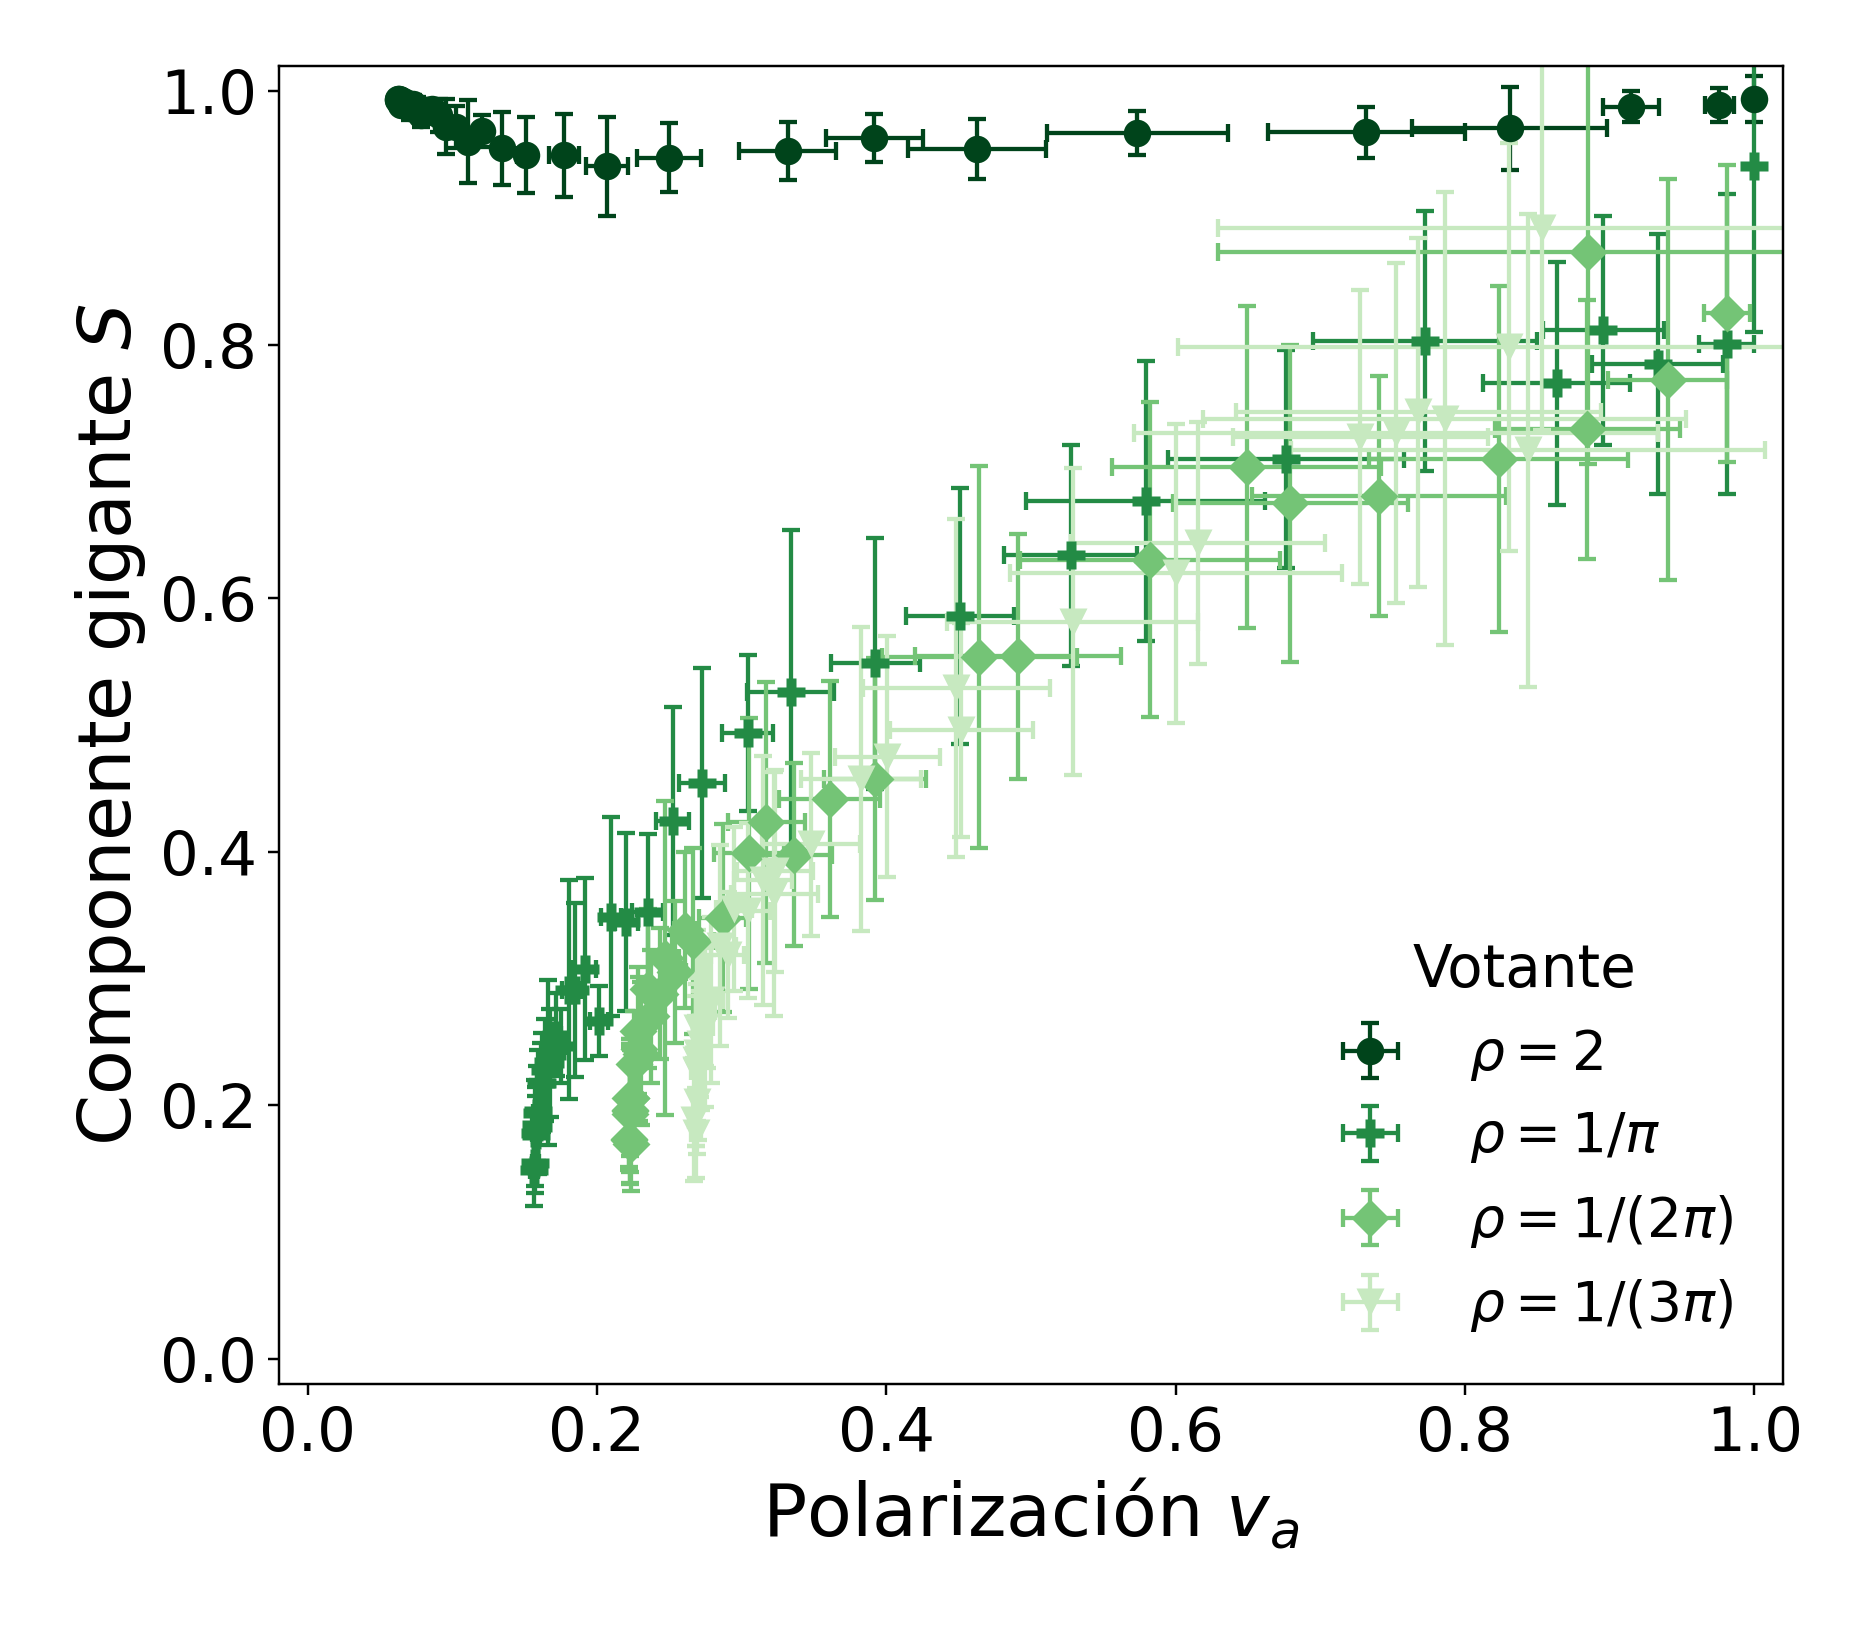
\includegraphics[width=\linewidth]{figs/image13b.png}
\end{minipage}
\caption{Polarización estacionaria en función de la componente gigante estacionaria para $\rho=2$ y las tres densidades bajas. Panel izquierdo: Vicsek. Panel derecho: votante. Cada punto corresponde a un $\eta$ del barrido.}
\label{fig:13}
\end{figure}

% ---------------------------------------------------------------------
\section{Tiempos de ejecución}
% ---------------------------------------------------------------------

Se comparó el tiempo de ejecución del Cell Index Method de este trabajo (C++) con el del TP1 (Búsqueda eficiente de partículas vecinas, Python con numpy). Se cronometró exclusivamente la búsqueda de vecinos, excluyendo generación de partículas, escritura de archivos y graficación. Parámetros comunes: $L=20$, $r_c=1$, contorno periódico, $N$ entre $10$ y $800$ (incluidos $200$, $400$ y $800$), $100$ repeticiones por punto, mismo equipo y sesión de trabajo para ambos motores. No se descartó ninguna repetición ni se aplicó un criterio de valor atípico; no fue necesaria una fase de calentamiento porque ninguna implementación conserva estado entre llamadas al CIM.

El TP1 usa partículas con radio no nulo ($r$ en $[0.23,0.26]$, sin superposición) y criterio de vecindad borde a borde, mientras que en este trabajo las partículas son puntuales con criterio centro a centro. Para separar el efecto de esta diferencia geométrica del efecto del lenguaje, se midieron tres condiciones: (A) TP1 tal como está construido, con radio; (B) una variante del mismo código de TP1 con radio igual a cero, que deja el mismo criterio centro a centro que este trabajo; y (C) el motor de este TP2. Cada condición usó la cantidad máxima de celdas por lado válida para su propio criterio ($13$ para A, $20$ para B y C), sin forzarlas a coincidir, porque esa diferencia forma parte de lo que se busca explicar.

La Fig.~\ref{fig:14} presenta el tiempo de búsqueda en función de $N$, junto con el número medio de vecinos por partícula. El motor de este TP2 resultó más rápido que ambas variantes del TP1 en todo el rango medido, aunque la diferencia no es constante: cercana a $90$ veces en $N=10$ y de aproximadamente $4.8$ veces en $N=800$. Una explicación posible es que a $N$ chico predomina un costo fijo por llamada (construcción de arreglos y overhead del intérprete en Python, ausente en código compilado), mientras que a $N$ grande predomina el trabajo de comparar pares candidatos, donde la diferencia se reduce porque la búsqueda de vecinos del TP1 ya está vectorizada con numpy.

\begin{figure}[H]
\centering
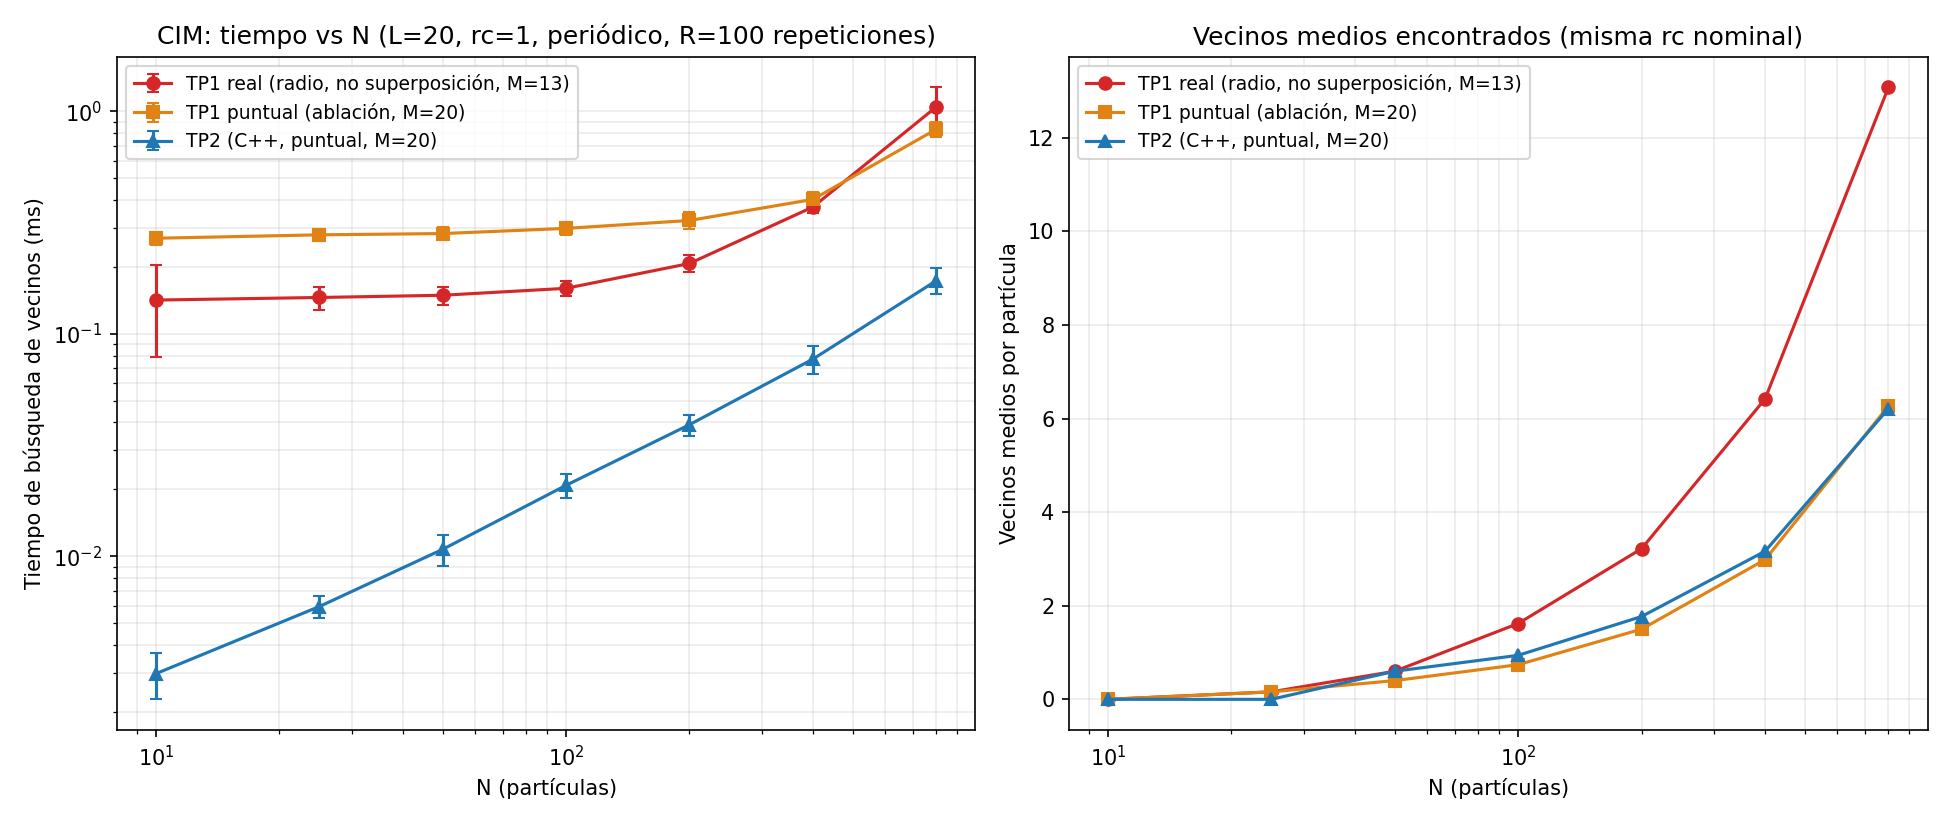
\includegraphics[width=0.95\linewidth]{figs/image14.png}
\caption{Tiempo de búsqueda de vecinos por CIM en función de $N$ (izquierda) y número medio de vecinos encontrados por partícula (derecha), para el TP1 con radio no nulo, el TP1 con partículas puntuales y el TP2. $L=20$, $r_c=1$, condición periódica, $100$ repeticiones por punto.}
\label{fig:14}
\end{figure}

Dentro del propio TP1, la condición con radio resultó más lenta que la variante puntual a partir de $N \approx 200$ (aproximadamente un $26\%$ más lenta en $N=800$). El número medio de vecinos encontrados a igual $r_c$ nominal fue de aproximadamente $13$ por partícula con radio y de aproximadamente $6$ en las dos condiciones puntuales, coincidentes entre sí. Esto es consistente con que el radio extiende el alcance efectivo de interacción y reduce la cantidad máxima de celdas por lado utilizable, aumentando la cantidad de partículas por celda y de pares candidatos comparados. La restricción de no superposición del TP1 no se refleja en estos tiempos porque la generación quedó excluida de la ventana cronometrada; su efecto es limitar la cantidad máxima de partículas generables para un $L$ dado, no la velocidad de cada búsqueda. Del mismo modo, que el TP1 mida un único estado estático no introduce una asimetría en esta comparación, porque en el TP2 la búsqueda de vecinos también se aisló del resto del motor de simulación.

% ---------------------------------------------------------------------
\section{Conclusiones}
% ---------------------------------------------------------------------

El estudio de la polarización muestra que ambos modelos pueden desarrollar orden direccional cuando el ruido es suficientemente bajo, pero difieren de manera marcada en su robustez frente a las perturbaciones angulares. En el modelo de Vicsek, la polarización disminuye gradualmente al aumentar $\eta$ y se mantiene elevada en un intervalo de ruido más amplio. Para la mayor parte del régimen ordenado, las simulaciones con mayor densidad conservan valores más altos de $v_a$, lo cual es consistente con el promedio vectorial de un vecindario más poblado. A ruido alto, las tres densidades convergen a valores bajos de polarización.

El modelo de votante es más sensible al ruido: para observar regímenes comparables de orden, valores intermedios y desorden fue necesario utilizar valores de $\eta$ mucho menores que en Vicsek. Sus series temporales exhiben además una dispersión mayor entre realizaciones en el régimen intermedio. En las simulaciones realizadas, el ordenamiento con la densidad es opuesto al de Vicsek: $\rho = 2$ conserva, en general, valores de $v_a$ superiores a $\rho = 4$ y $\rho = 8$. Este resultado se reporta como una tendencia empírica del protocolo empleado, ya que el estudio no separa de manera independiente los efectos de densidad y del tamaño del sistema $N$.

La comparación directa confirma que el promedio vectorial de las orientaciones vecinas en Vicsek amortigua las fluctuaciones y permite sostener el orden colectivo a ruidos más altos que la regla de copia aleatoria del votante. Asimismo, las configuraciones características muestran que la conectividad geométrica y el orden direccional son observables distintos: una componente gigante grande, medida por $S$, no implica necesariamente una polarización alta. Finalmente, los cambios observados en el régimen intermedio describen una competencia entre alineación y ruido, pero las simulaciones presentadas no permiten estimar un punto crítico ni caracterizar una transición de fase.

% ---------------------------------------------------------------------
\section*{Referencias}
% ---------------------------------------------------------------------

\begin{enumerate}
\item[{[1]}] Vicsek, T., Czirók, A., Ben-Jacob, E., Cohen, I., \& Shochet, O. (1995). Novel type of phase transition in a system of self-driven particles. \textit{Physical Review Letters}, 75(6), 1226.
\item[{[2]}] Loscar, E. S., Baglietto, G., \& Vazquez, F. (2021). Noisy multistate voter model for flocking in finite dimensions. \textit{Physical Review E}, 104(3), 034111.
\end{enumerate}

\end{document}
